\documentclass[12pt, letterpaper, oneside]{book}
%\documentclass[12pt, letterpaper]{book}

\usepackage[spanish,es-tabla]{babel}
\usepackage[utf8x]{inputenc}
\usepackage{microtype}
\usepackage{emptypage}
\usepackage{usmtesis}
\usepackage{url}
\usepackage{caption}
\usepackage{amsmath}
\usepackage{listings}
%\usepackage{graphicx}
\usepackage{subcaption}
\usepackage{cite}
\usepackage{amsfonts}
\usepackage{algorithm}
\usepackage[noend]{algpseudocode}
\usepackage[nottoc,notlot,notlof]{tocbibind}
\usepackage{tikz}
\usetikzlibrary{babel,arrows.meta,shapes,arrows,patterns}
\usepackage{pgfplots}
\usepgfplotslibrary{dateplot}
\usepackage{pgfplotstable}

\lstset{basicstyle=\ttfamily\small, numbers = left}

%\usepackage{layout} %debug only

\RequirePackage{fancyhdr}
\newcommand{\hsp}[1][20]{\hspace{#1pt}}
\fancyhf{}
\fancypagestyle{plain}{%
	\fancyhf{} 
	\fancyhead[L]{\scriptsize \rightmark}
	\fancyhead[R]{\scriptsize \leftmark}
	\fancyfoot[R]{\bfseries \thepage}
	\fancyfoot[L]{Departamento de Informática. UTFSM.}
	\renewcommand{\headrulewidth}{0.1pt}
	\renewcommand{\footrulewidth}{0.1pt}
}
%\setlength{\footheight}{110pt} 

%macros
\renewcommand{\tt}[1]{\texttt{#1}}
\renewcommand{\it}[1]{\textit{#1}}
\renewcommand{\bf}[1]{\textbf{#1}}
\newcommand{\etal}{\emph{et al.}}
\newcommand{\get}{$\gets$\,\,}
\newcommand{\ra}{$\rightarrow\,\,$}
\newcommand{\la}{$\leftarrow\,\,$}

\floatname{algorithm}{Algoritmo}
\renewcommand{\listalgorithmname}{Índice de algoritmos}
\renewcommand{\algorithmicrequire}{\textbf{Input:}}
\renewcommand{\algorithmicensure}{\textbf{Output:}}


\begin{document}
\frontmatter
\thispagestyle{empty}
%!TEX root = main.tex

\begin{center}
  \begin{spacing}{1}
    {\large UNIVERSIDAD TÉCNICA FEDERICO SANTA MARÍA}\\
    DEPARTAMENTO DE INFORMÁTICA\\
    VALPARAÍSO - CHILE
  \end{spacing}

  \vspace{12mm}
  \includegraphics[height=50mm]{figures/utfsm.pdf}
  \vspace{15mm}

  \begin{spacing}{1.5} 
    %\textbf{\large ANÁLISIS DE CONSULTAS A BASE DE DATOS DE GRAFOS RDF}\\
    %\textbf{\large CASO DE USO: DATOS BIOLÓGICOS}\\
    \textbf{\large ANÁLISIS DE CENTRALIDAD DE BASE DE DATOS RDF }\\
    \textbf{\large CASO DE USO: DATOS BIOLÓGICOS }\\
  \end{spacing}

  \vspace{20mm}
  \textbf{\large HERNÁN FELIPE VARGAS LEIGHTON}
  \vspace{12mm}

  \begin{spacing}{1.25} 
    %MEMORIA PARA OPTAR AL TÍTULO DE\\
    %INGENIERO CIVIL EN INFORMÁTICA
    PRIMER AVANCE DE MEMORIA
  \end{spacing}

  \vspace{15mm}
  \begin{table}[h]
    \begin{center}
      \begin{tabular}{ l c l }
        PROFESOR GUÍA & : & CARLOS BUIL A.\\
        PROFESOR CORREFERENTE & : & CECILIA REYES C.\\
      \end{tabular}
    \end{center}
  \end{table}

  \vfill
  \large ENERO 2016
\end{center}

\newpage

%debug
%\layout
%\newpage

%% Hack para el abstract corregir si se puede.
%\chapter*{ }
%\vspace{-3cm}
%\section*{Abstact} \chaptermark{Abstract}
%\section*{Resumen}

\begin{spacing}{1}
  \tableofcontents \chaptermark{Tabla de contenidos}
  \listoffigures
  \listoftables
  \listofalgorithms
\end{spacing}

\mainmatter

%!TEX root = main.tex

\chapter{Introducción}\label{ch:intro}

La Web actual está hecha por y para las personas. Desde las publicaciones en las
redes sociales hasta los artículos más avanzados en las enciclopedias virtuales
son formas de transferir información entre individuos y por ello utilizan el
lenguaje natural para hacer más fácil su entendimiento. Si bien estas
características facilitan la comprensión para el ser humano, hacen cada
vez más difícil el manejo de estos datos por parte de los computadores debido a
la falta de un lenguaje común, lo que las obliga a intentar interpretar el
contexto y la intencionalidad del emisor, todo esto sumado a la masividad de la
información publicada hoy en día, donde todos pueden publicar lo que quieran y
en cualquier formato.

La Web Semántica nace como forma de solucionar esta problemática.
Su objetivo es que las máquinas puedan generar e intercambiar datos por Internet 
de manera que estos sean interpretables y procesables de forma simple tanto por
las personas como por otros computadores.
Esto implica que los datos deben tener un modelo común, compatible y general,
y además, una visualización acorde para facilitar la lectura de los mismos por
los seres humanos.

Uno de los pilares fundamentales para la creación de una Web en la cual toda
información pueda ser accedida por computadores de manera rápida y efectiva es
la generación de datos enlazados, es decir, la publicación e integración del 
conocimiento existente a un modelo que permita la interconexión y extensión de
los datos sin limitar el dominio ni las relaciones de los mismos.

Tim Berners-Lee, el inventor de la Web, propulsor de la Web Semántica,
y fundador del \emph{World Wide Web Consortium} el cual ha generado estándares
que ayudan a solucionar este problema como son RDF, SPARQL entre otros;
propone una clasificación de cinco estrellas para los datos publicados:
\begin{enumerate}
  \item
    Publica tus datos en la Web, con cualquier formato y una licencia abierta.
  \item
    Utiliza datos estructurados (tablas, antes de imágenes de las mismas, etc).
  \item
    Utiliza formatos no propietarios.
  \item
    Utiliza URIs para denotar las cosas de manera que la gente pueda apuntar a
    ellas\footnote{
    Una forma de hacerlo es con URL, links a páginas Web por ejemplo, de manera
    que otras personas puedan revisar el contenido y enlazar con él.}.
  \item
    Enlaza tus datos con otros para proveer contexto.
\end{enumerate}

Siguiendo los estándares y las recomendaciones hechas por Tim Berners-Lee se han
creado variados proyectos.
Actualmente existe una gran cantidad de datos de libre acceso enlazados en la
Web. La figura \ref{fig:cloud} muestra un esquema de ellos y provee una visión
global de los diferentes tópicos que estos datos tratan, ya sean datos
geográficos, de redes sociales, biológicos o lingüísticos (entre otros).

En este trabajo nos enfocaremos en los datos biológicos, en particular a partes
del proyecto Bio2RDF\cite{belleau2008bio2rdf}.
Dicho proyecto (en su \emph{release} 3) incorpora la información de 35 bases de
datos RDF con información biológica, cerca de 11.000 millones de triples que
conforman la red de datos enlazados más grande de esta ciencia.

En trabajos anteriores como en Hu \emph{et al.}\cite{hu2015link} se han
determinado parámetros como el grado de distribución, la simetría y la
transitividad de los enlaces entre las diferentes bases de datos que lo
componen, además de la existencia del fenómeno conocido como ``mundo pequeño'',
lo que significa que, a pesar del gran número de nodos que existen en esta red
de datos, generalmente es posible encontrar un camino relativamente corto entre
ellos.

Un investigador podría estar interesado en verificar si existe alguna relación
entre los componentes químicos de las drogas utilizadas para combatir la
obesidad y aquellas que se usan en contra de la diabetes.
El proyecto Bio2RDF le ayudará en este cometido ya que enlaza grandes bases de
datos de las ciencias biológicas como aquellas de enfermedades, medicamentos,
química y muchas más.

Pero, ¿Cuáles son los datos más importantes para los usuarios?, ¿Cómo se
relacionan entre ellos? Son interrogantes que se presenta naturalmente al
momento de evidenciar la cantidad abrumadora de datos enlazados existentes.
En este trabajo responderemos dichas interrogantes para parte de los datos de
Bio2RDF, en específico la base de datos DrugBank, la cual no solo es de las más
consultadas del proyecto, sino que además posee algunos de los datos más
interesantes de esta ciencia como son los medicamentos.

\begin{figure}[ht]
  \centering
  \includegraphics[width=\textwidth]{figures/open_linked_data_could.png}
  \caption{Conexiones entre las bases de datos abiertas hasta agosto del 2014.}
  \vspace{-.2cm}
  \caption*{\small
    En morado las bases de datos biológicas, gran parte de ellas son parte del
    proyecto Bio2RDF.
    Imagen creada por Linked Open Data Cloud project\cite{lod:cloud}.}
  \label{fig:cloud}
\end{figure}
~\vspace{-1cm}

\section{Identificación del problema}\label{sec:idpro}
Debido al volumen de datos que se maneja en el proyecto Bio2RDF, se vuelve
interesante determinar cuál es la información más importante consultada por
parte de los usuarios y así verificar el soporte que ésta tiene en el modelo. 
Para ello es indispensable contar con métricas que analicen el uso de los datos
consultados, la relevancia y la relación entre los mismos.

Actualmente no existe un estudio que determine cuál es el subconjunto de datos
que realmente son utilizados y por ello no es posible verificar cuáles son
las entidades más importantes dentro de este proyecto.

Además sabemos que el fenómeno de ``mundo pequeño'' que presenta Bio2RDF, es
generalmente evidenciado en las redes sociales. En éstas se 
teoriza que dos individuos cualquiera están relacionados entre si por un número
pequeño de pasos, como describe la hipótesis de los seis grados de separación o
muestra el estudio ``Anatomy of Facebook''\cite{ugander2011anatomy}.

Esta característica evidencia la existencia de individuos claves en la
comunicación de una red social. 
Una de las métricas más utilizadas y con mejores resultados para determinar
estos individuos es el análisis de centralidad.

La centralidad es una forma de medir la importancia de un nodo en una red.
En las redes sociales se transforma en una medida de la influencia de una
persona con respecto a sus pares, en redes de transporte puede identificar los
puntos críticos y cuellos de botella, y de la misma manera, en una red RDF
esperamos que señale los datos más importantes.

Debido a estas características consideramos atractivo generar un cálculo de
centralidad para los datos consultados por los usuarios al proyecto Bio2RDF,
específicamente a una de las bases de datos que presenta mayor cantidad de
consultas en él: DrugBank, y así identificar tanto cuáles son las
instancias más importantes como las relaciones claves existentes en ella.

\section{Objetivos}\label{sec:objs}

El objetivo de este trabajo es generar estadísticas de centralidad sobre el
subconjunto de datos consultados por los usuarios a la base de datos DrugBank,
parte importante del proyecto Bio2RDF.
Se espera lograr determinar cuáles son los miembros claves de esta base de datos
y verificar si los resultados son congruentes con el modelo de datos planteado
por el proyecto.

\subsection{Objetivos específicos}\label{sec:objs:esp}
Para el logro del objetivo general se plantean los siguientes objetivos
específicos:
\begin{enumerate}
  \item
    Generar un subgrafo del proyecto Bio2RDF a través del análisis de las
    consultas SPARQL hechas al servidor por parte de los usuarios en un periodo
    de tiempo determinado.
  \item
    Analizar el grafo generado por medio de métricas de centralidad para grafos.
  \item
    Comparar los resultados del estudio con el proyecto Bio2RDF.
\end{enumerate}

%!TEX root = main.tex

\chapter{Estado del arte}
El proyecto Bio2RDF utiliza las tecnologías de la Web Semántica para su
implementación y funcionamiento. Así, el análisis que se hará en esta memoria
toma estos conocimientos como base y generará a través de ellos estadísticas de
centralidad con las cuales se determinará cuales son los datos más importantes
de dicha base de datos.

Para poder analizar el problema correctamente es necesario el conocimiento de
las tecnologías que se enuncian en este capítulo. En la sección \ref{ea:ws} se
describe qué es la Web Semántica y las tecnologías que la componen.
En la sección \ref{ea:bio} se hace una revisión al proyecto Bio2RDF y a las
bases de datos que forman parte de él, en especial a la utilizada en este
documento: DrugBank; y en la sección \ref{ea:cent} se repasan conceptos básicos
de teoría de grafos y se introduce el concepto de centralidad junto a sus
métricas y algoritmos.

\section{Web Semántica}\label{ea:ws}
La Web Semántica es un conjunto de actividades propuestas por la \emph{World
Wide Web Consortium} (desde ahora W3C) con el objetivo de generar tecnologías
para la publicación de datos en la web de tal manera que sean procesables por
las maquinas. 
Se basa en la idea de añadir metadatos semánticos y ontológicos que describan el
contenido y la relación entre los datos publicados. De esta manera se logra
mejorar la interoperatividad de internet pues los programas podrán acceder a los
datos en un lenguaje formal, procesar su contenido, razonar en base a este y
%TODO: formal: no es que sea formal, todos los lenguajes lo son de alguna forma,
%es que todo tiene el mismo modelo de datos y los mismos vocabularios (que no
%lenguajes)
combinarlo para resolver problemas cotidianos automáticamente.

Es posible rastrear los orígenes de esta idea hasta una propuesta temprana de la
\emph{World Wide Web} en 1986~\cite{berners1989proposal} y el subsecuente
trabajo de Berners-Lee \etal\cite{berners1992world} donde se prevé la
necesidad de una evolución desde objetos legible por las personas a información
semántica orientada a las máquinas.

Para lograr los objetivos de la Web Semántica se han generado múltiples
metalenguajes y estándares de representación como son XML, XML Schema, RDF,
RDF Schema, OWL y SPARQL. Estas tecnologías se utilizan actualmente para generar
datos enlazados (\emph{Linked Data}), que buscan enlazar información arbitraria
en la web generando así una ``\emph{red de las cosas del mundo, descrita por los
datos en la Web}''\cite{berners2011linked}.

\begin{figure}[htpb]
  \centering
  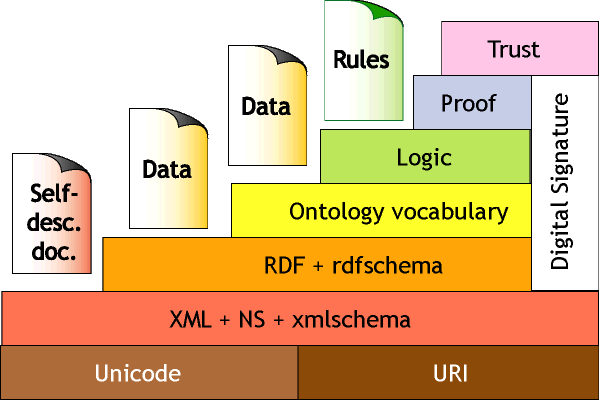
\includegraphics[width=.6\textwidth]{figures/Semantic_web_stack.png}
  \caption{Pila de tecnologías de la Web Semántica.}
  \vspace{-.25cm}
  \caption*{Creado por Marobi1\cite{wikimg:swstack}.}
  \label{fig:swstack}
\end{figure}

En las siguientes secciones se describirán más detalladamente algunos de los
conceptos presentados en la figura \ref{fig:swstack} comenzando desde la base,
con las tecnologías del hipertexto (URI y XML), para luego pasar a las
tecnologías de la Web Semántica más estandarizadas (RDF, RDFS y OWL) y terminar
con el lenguaje de consulta SPARQL.

\subsection{URI}
Una URI (del las siglas del ingles \emph{Uniform Resource Identifier}) es una
cadena de caracteres utilizada para identificar un recurso inequívocamente.
Si bien en un principio solo acepta un subconjunto caracteres ASCII (el alfabeto
en ingles y los números) y ``código porciento'' (en el cual, por ejemplo '\%26'
es '\&') el estándar fue extendido el 2005 a IRI (\emph{Internationalized
resource identifier}) que puede contener caracteres Unicode/ISO 10646,
incluyendo chino, japones, koreano, entre otros\cite{gangemi2006bourne}.
En este documento no se diferenciará entre URI e IRI.

La sintaxis actual de una URI fue definida por Berners-Lee et al. el
2005 ~\cite{berners2004uniform} como sigue:\\
\texttt{
  scheme:{[//{[user:passwd@]}host{[:port]}]}{[/]}path{[?query]}{[\#frag]}
}\\
donde:
\begin{itemize}
  \item
    El \bf{esquema} (\emph{scheme}) que consiste en una secuencia de caracteres
    sensibles a las mayúsculas que comienza con una letra y es seguido por
    cualquier combinación de letras, puntos (\tt{.}), guiones (\tt{-}) y signos
    más (\tt{+}), terminando con dos puntos (\tt{:}). 
    Ejemplos populares son \tt{http:}, \tt{ftp:} y \tt{mailto:}.
  \item
    Las dos barras (\tt{//}) son requeridos para algunos esquemas. Cuando la
    componente de autoridad no está presente la ruta no puede comenzar con dos
    barras.
  \item
    La \bf{autoridad} se divide como sigue:
    \begin{itemize}
      \item
        Una \bf{autentificación} opcional compuesta por el usuario
        (\emph{user}), dos puntos y una contraseña (\emph{password}) terminando
        en un arroba (\tt{@}).
      \item
        Un anfitrión (\emph{host}) que puede ser un nombre registrado un una
        dirección IP.
      \item
        Un número de \bf{puerto} opcional (\emph{port}) separado del anfitrión
        por dos puntos.
    \end{itemize}
  \item
    Una \bf{ruta} (\emph{path}) que es una secuencia de segmentos separados
    por una barra (\tt{/}) que comienza con una de las mismas. Generalmente
    representa la localización de un archivo en un sistema de archivos
    jerárquico pero no es necesario.
  \item
    Una \bf{consulta} opcional (\emph{query}) que comienza con un signo de
    interrogación (\tt{?}) y, a pesar de no tener un sintaxis claramente
    definida, usualmente presenta pares atributo-valor.
  \item
    Un \bf{fragmento} opcional (\emph{fragment}) que comienza con un numeral
    (\tt{\#}) seguido por un identificador secundario al recurso principal.
\end{itemize}

\begin{figure}[htpb]
  $$
    \underbrace{\text{http}}_{\text{esquema}}\text{://}
    \overbrace{
      \overbrace{
        \underbrace{\text{user:password}}_{\text{autentificación}}\text{@}
        \underbrace{\text{example.com}}_{\text{anfitrión}}\text{:}
        \underbrace{\text{80}}_{\text{puerto}}
      }^{\text{autoridad}}
      \overbrace{\text{/path/data}}^{\text{ruta}}
    }^{\text{parte jerárquica}}\text{?}
    \underbrace{\text{key=value}}_{\text{consulta}}\text{\#}
    \underbrace{\text{section1}}_{\text{fragmento}}
  $$
  \caption{Ejemplo de una URI.}
  \label{fig:uriex}
\end{figure}

Un ejemplo de lo anterior sería la figura \ref{fig:uriex} donde podemos notar
que una URL (\emph{Uniform Resource Locator}) es una URI, pero no debemos
confundir los términos pues una URL además de identificar un recurso web permite
obtener una representación del mismo generalmente en formato HTML vía HTTP. Es
decir, una URL es una URI que apunta a un recurso físico en la web, mientras que
una URI no necesariamente debe apuntar a una localización que exista realmente.

\subsection{XML}
XML es el acrónimo del ingles \emph{Extensible Markup Language}. Es un
lenguaje de marcado desarrollado por el W3C para almacenar datos de manera
legible tanto por personas como por máquinas. 
El diseño de XML busca la simplicidad, generalidad y usabilidad a través de
internet\cite{paoli2004extensible}. 

Un documento XML puede comenzar con un identificador declarando alguna
información sobre el documento en sí. Luego el cuerpo del fichero debe contener
solo un elemento raíz y dentro de éste se pueden escribir múltiples elementos y
atributos.

\begin{figure}[htpb]
  \centering
  \begin{tabular}{c}
    \lstinputlisting[
      basicstyle=\ttfamily\scriptsize,
      language=xml]{code/example-xml.xml}
  \end{tabular}
  \caption{Ejemplo de XML.}
  \vspace{-.25cm}
  \label{fig:xmlex}
\end{figure}

En la figura~\ref{fig:xmlex} vemos la libertad que nos da XML a la hora de
representar cualquier tipo de información, pero esta libertad hace que
interpretar la validez de un documento sea complicado, pues la información
contenida en este puede ser sensible a la aplicación y el lenguaje definido con
esta tecnología. En respuesta a esta problemática el W3C desarrolló \emph{XML
Schema} que cobra vital importancia para la Web Semántica.

\subsection{XSD}
XSD (del ingles \emph{XML Schema Definition}) es una recomendación del W3C que
especifica formalmente la estructura y restricciones de los contenidos de un
fichero XML de manera precisa más allá de las normas sintácticas del propio
lenguaje XML.

A diferencia de otros lenguajes de esquemas para XML, XSD especifica también
tipos de datos y sus restricciones, logrando un estándar a la hora de
representar datos~\cite{biron2004xml}. 
Presenta 19 tipos de datos básicos: \tt{anyURI},
\tt{base64Binary}, \tt{boolean}, \tt{date}, \tt{dateTime}, \tt{decimal},
\tt{double}, \tt{duration}, \tt{float}, \tt{hexBinary}, \tt{gDay}, \tt{gMonth},
\tt{gMonthDay}, \tt{gYear}, \tt{gYearMonth}, \tt{NOTATION}, \tt{QName},
\tt{string} y \tt{time}. Además permite la creación de nuevos tipos de datos por
medio de tres mecanismos:
\begin{itemize}
  \item \bf{Restricción:} Reduce los valores que puede tomar un dato.
  \item \bf{Lista:} Permite una secuencia de valores.
  \item \bf{Unión:} Permite la elección de valores de diferentes tipos.
\end{itemize}

Gracias a estos factores un fichero XML Schema puede representar un modelo de
datos completo y robusto, con relaciones entre las entidades y asignaciones de 
tipos de datos básicos. La figura~\ref{fig:xsdex} muestra un ejemplo del uso de
XML en conjunto con XSD.

Esta característica es fundamental para la Web Semántica pues todos los tipos de
datos de XSD son compatibles con RDF.

\begin{figure}[htpb]
  \centering
  \begin{tabular}{c}
    \lstinputlisting[
      basicstyle=\ttfamily\scriptsize,
      language=xml]{code/example-xmls.xml}
  \end{tabular}
  \caption{Ejemplo de XMLS.}
  \vspace{-.25cm}
  \caption*{Definiendo una película con XSD.}
  \label{fig:xsdex}
\end{figure}

\subsection{RDF}\label{sw:rdf}
RDF (del inglés \emph{Resource Description Framework}) es una familia de
especificaciones del W3C diseñada como un modelo de datos para metadatos.
Fue adoptado como una recomendación del W3C en 1999, mientras que la
especificación 1.0 fue publicada el 2004 y la 1.1 el
2014\cite{bikakis2013semantic}.

El modelo de datos RDF se basa en la idea de hacer declaraciones sobre 
recursos web (URIs) en forma de expresiones $\langle sujeto, predicado, objeto
\rangle$ que son llamados triples RDF.
El $sujeto$ indica el recurso mientras que el $predicado$ denota la relación
con el $objeto$.
Digamos $U$ un conjunto de URIs, $B$ un conjunto de recursos anónimos y $L$ un
conjunto de literales XSD, podemos denotar un triple RDF como 
$\langle s,p,o\rangle \in (U\cup B) \times U \times (U\cup B\cup L)$.
Así podemos decir que un triple RDF sigue la clásica notación \tt{entidad} - 
\tt{atributo} - \tt{valor} de los modelos orientados a objetos, permitiendo
además, gracias a su simpleza, modelar todo tipo de conceptos abstractos.

Llamaremos vocabulario a la definición de conceptos y relaciones (términos)
utilizados para describir y representar un área de conocimiento.
Otro concepto a tener en cuenta son las ontologías, aunque no existe una clara 
división entre éstas y los vocabularios, generalmente se les considera más
complejas y formales.
En la Web Semántica una colección de triples RDF puede denotar un vocabulario o
ontología.

El vocabulario incluido en la especificación RDF es muy básico y por ello fue
extendido a \emph{RDF Schema}, por lo que la gran mayoría de las bases de datos
RDF actuales contienen ambos vocabularios.

Un conjunto de triples RDF será representado naturalmente por un grafo dirigido.
Esta característica faculta la tecnología para ser parte fundamental de la web 
semántica pues permite relacionar información de diferentes fuentes sin mayor
problema y representarla en un esquema fácilmente identificable.

RDF es un modelo abstracto con varios formatos de serialización, por lo que la
codificación de un triple varía dependiendo el tipo de archivo en el que se
guarde. En esta memoria se trabajará con triples codificados en RDF/XML,
Turtle\cite{beckett2014turtle} y N-Triples\cite{beckett2014nt}.

RDF/XML fue la primera codificación estándar para serializar RDF (en un archivo
XML) y si bien es potente, es difícil de leer por las personas. En base a esto
utilizaremos Turtle y N-Triples pues su simpleza los hace ideales para el
entendimiento y procesamiento de los triples.

Algunas de las reglas para escribir un archivo Turtle (\tt{.ttl}) son las
siguientes:
\begin{itemize}
  \item Toda sentencia termina con un punto (\tt{.}).
  \item La sucesión de tres URIs es un triple.
  \item 
    Si una linea termina en punto y coma (\tt{;}) la siguiente linea mantiene el
    $sujeto$ y solo es necesario escribir las URIs del $predicado$ y el
    $objeto$.
  \item 
    Se pueden definir prefijos con \tt{@prefix rdf: <some\_URI> .}. Esta
    característica es particularmente útil para agregar vocabularios ya
    definidos.
\end{itemize}

N-Triples es una subsección del lenguaje Turtle y su característica principal es
la facilidad que presenta a la hora de analizar su sintaxis. En un archivo
N-Triples (\tt{.nt}) solo se pueden escribir tres URIs seguidas de un punto para
representar un triple RDF y todo lo que esté después de un numeral (\tt{\#}) se
considera un comentario.

Podemos encontrar una descripción completa de las características y sintaxis de
Turtle en~\cite{beckett2014turtle}, de N-Triples en~\cite{beckett2014nt} y de
RDF/XML en ~\cite{beckett2004rdf}.

En la figura \ref{fig:triples} podemos ver un ejemplo básico de la utilización 
de Turtle para la generación de triples (figura \ref{fig:triples:ttl}), el
mismo ejemplo escrito en XML/RDF (figura \ref{fig:triples:rdf}) y como estos
pueden ser visualizados como un grafo dirigido (\ref{fig:triples:grafo}).
\begin{figure}[htpb]
  \centering
  \begin{subfigure}[b]{\textwidth}
    \centering
    \begin{tabular}{c}
      \lstinputlisting[basicstyle=\ttfamily\scriptsize]{
        code/example-turtle.ttl}
    \end{tabular}
    \caption{Ejemplo en Turtle.}
    \label{fig:triples:ttl}
  \end{subfigure}
  \\[0.5cm]
  \begin{subfigure}[b]{\textwidth}
    \centering
    \begin{tabular}{c}
      \lstinputlisting[basicstyle=\ttfamily\scriptsize]{
        code/example-xml-rdf.rdf}
    \end{tabular}
    \caption{Mismo ejemplo en XML/RDF.}
    \label{fig:triples:rdf}
  \end{subfigure}
  \\[0.5cm]
  \begin{subfigure}[]{\textwidth}
    \centering
    \begin{tikzpicture}
  \begin{scope}[every node/.style={ellipse,thick,draw,font=\small}]
    \node (A) at (0,0)    {ex:utfsm};
    \node (B) at (6,1.5)  {ex:universidad};
    \node (C) at (6,0)    {ex:federico};
    \node (D) at (6,-1.5) {http://www.usm.cl};
    \node (E) at (12.5,0) {Federico Santa Maria};
  \end{scope}
  \begin{scope}[>={Stealth[black]},
                every node/.style={font=\footnotesize},
                every edge/.style={draw=black,very thick}]
    \path[->] (A) edge [sloped, above]   node {rdf:type}      (B);
    \path[->] (A) edge [above]           node {ex:fundador}   (C);
    \path[->] (A) edge [sloped, below]   node {ex:pagina}     (D);
    \path[->] (C) edge [above, pos=0.45] node {ex:nombre}     (E);
  \end{scope}
\end{tikzpicture}

\begin{tikzpicture}
  \begin{scope}[every node/.style={ellipse,thick,draw,font=\small}]
    \node (A) at (0,0)  {ex:fundador};
    \node (B) at (0,-1.5) {ex:nombre};
    \node (C) at (5,-0.75) {rdf:Property};
  \end{scope}
  \begin{scope}[>={Stealth[black]},
                every node/.style={font=\footnotesize},
                every edge/.style={draw=black,very thick}]
    \path[->] (A) edge [sloped, above]   node {rdf:type}      (C);
    \path[->] (B) edge [sloped, above]   node {rdf:type}      (C);
  \end{scope}
\end{tikzpicture}

    \caption{Grafo generado.}
    \label{fig:triples:grafo}
  \end{subfigure}
  \caption{Ejemplo de triples RDF.}\label{fig:triples}
\end{figure}

\subsection{RDFS}
RDFS (de las siglas del ingles \emph{Resource Description Framework Schema},
también llamado RDF Schema) es un vocabulario que extiende RDF proveyendo un
set de clases y propiedades que mejoran la creación de modelos como son:
\tt{Class} para declarar clases, \tt{subClassOf} para denotar herencia,
\tt{range} y \tt{domain} para el rango y dominio de cierta propiedad
(\tt{rdf:Property}), entre otras.

RDF fue presentado en 1998 e introducido finalmente como recomendación del W3C
el 2004\cite{bikakis2013semantic}.

RDFS provee el vocabulario necesario para la construcción de cualquier ontología
más avanzada y por ello es la base de otros vocabularios del como OWL y SKOS.

La especificación completa del vocabulario puede encontrarse en ~\cite{brickley2014rdfs}.
%en https://en.wikipedia.org/wiki/RDF_Schema#RDFS_entailment hay un ejemplo.

\subsection{OWL}
OWL (del ingles \emph{Web Ontology Language}) es una familia de lenguajes para
la creación de ontologías complejas.
Agrega lógica computacional para que las relaciones
hechas con este lenguaje puedan ser procesadas con el fin de verificar la
consistencia de la información o generar información implicita.

La versión actual de OWL se conoce como ``OWL 2'' y fue publicada el 2009 como 
una revisión y extensión de la versión inicial publicada el
2004\cite{bikakis2013semantic}. Generalmente cuando se hablar de ``OWL'' nos
referimos a la versión del 2004.

Actualmente OWL tiene tres variantes (sublenguajes) enumerados del más simple al
más complejo como sigue\cite{mcguiness2004owl}:
\begin{enumerate}
  \item \bf{OWL Lite}:
    Se ideó pensando en dar soporte a restricciones simples y jerarquía básica,
    por ejemplo la cardinalidad de los números. 
    Se esperaba que fuera más facil generar y mantener herramientas para OWL
    Lite que para sus variantes más avanzadas, pero debido a que casi todas las
    características de OWL DL pueden ser implementadas como una combinación de
    las de OWL Lite, los desarrolladores han probado que no es 
    así\cite{grau2008owl}. Actualmente OWL Lite no es ampliamente utilizado.
  \item \bf{OWL DL}:
    Fue diseñado para proveer la máxima expresividad posible sin perder la
    decidibilidad y completitud computacional. Posee el vocabulario completo de
    OWL pero solo puede ser utilizado cumpliendo ciertas restricciones.
  \item \bf{OWL Full}:
    Fue diseñado para mantener la compatibilidad con RDFS, permite todo el
    vocabulario sin restricciones pero es indecidible por lo que un programa de
    razonamiento no puede asegurar la completitud de los resultados.
\end{enumerate}
Así, toda ontología o conclusión valida en OWL Lite tambien lo será en OWL DL y
estás a su vez lo serán en OWL Full.

OWL 2 tiene tres perfiles dependiendo de la función que cumple.
\begin{enumerate}
  \item \bf{OWL 2 EL}: 
    Es el fragmento del lenguaje decidible en tiempo polinomial, diseñado para
    trabajar con grandes volúmenes de propiedades y clases.
  \item \bf{OWL 2 QL}:
    Fue diseñado para facilitar el acceso a \emph{datasets} con un gran número
    de instancias donde las consultas son más importantes que el razonamiento.
  \item \bf{OWL 2 RL}:
    Está optimizado para el análisis de reglas lógicas, en aplicaciones que
    requieren un razonamiento escalable sin perder la expresividad del lenguaje.
\end{enumerate}
Se pueden ver las características completas de los perfiles de OWL 2 en
~\cite{motik2009owlprofiles}.

\subsection{SPARQL}
SPARQL (del ingles \emph{SPARQL Protocol and RDF Query Language}) es un lenguaje
estandarizado para consultar grafos RDF, se constituyó como una recomendación
oficial por la W3C en el 2008\cite{bikakis2013semantic}. La versión actual de
SPARQL es la 1.1\cite{world2013sparql}.

SPARQL provee un set completo de operaciones analíticas para sus consultas
definidas directamente en la especificación. Particularmente provee 4 formas de
consultas:
\begin{itemize}
  \item \bf{\tt{SELECT}}:
    Retorna valores en forma de tabla.
  \item \bf{\tt{CONSTRUCT}}:
    Retorna valores en forma de triples RDF.
  \item \bf{\tt{ASK}}:
    Retorna un resultado binario a la consulta (\tt{True/False}).
  \item \bf{\tt{DESCRIBE}}:
    Retorna un grafo RDF con contenido que el administrador del \emph{endpoint}
    SPARQL considere información útil.
\end{itemize}
A excepción de \tt{DESCRIBE}, las demás consultas necesitan un bloque \tt{WHERE}
con sintaxis similar a Turtle en el cual se determinan las restricciones de la
búsqueda en forma de triples RDF con variables y URIs.

Además de las consultas, SPARQL provee múltiples funciones como son 
las condicionales (\tt{if}, \tt{exists}, etc), de conversión (\tt{str},
\tt{lang}, etc), de comprobación (\tt{isNumber}, \tt{isBlank}, etc) y
modificadores de respuesta como \tt{ORDER BY}, \tt{DINSTINCT}, \tt{REDUCED},
\tt{LIMIT} y \tt{OFFSET}. Una descripción completa del lenguaje puede
encontrarse en ~\cite{prud2008sparql} y en ~\cite{world2013sparql}.

\begin{figure}[htpb]
  \centering
  \begin{subfigure}[b]{\textwidth}
    \centering
    \begin{tabular}{c}
      \lstinputlisting[basicstyle=\ttfamily\scriptsize]{
        code/example-select.sparql}
    \end{tabular}
    \caption{Ejemplo de consulta tipo \tt{SELECT}.}
    \label{fig:sparql:select}
  \end{subfigure}
  \\[0.5cm]
  \begin{subfigure}[b]{\textwidth}
    \centering
    \begin{tabular}{c}
      \lstinputlisting[basicstyle=\ttfamily\scriptsize]{
        code/example-construct.sparql}
    \end{tabular}
    \caption{Ejemplo de consulta tipo \tt{CONSTRUCT}.}
    \label{fig:sparql:construct}
  \end{subfigure}
  \caption{Ejemplo de consultas SPARQL.}\label{fig:sparql}
\end{figure}

En la figura~\ref{fig:sparql:select} se ve un ejemplo de una consulta SPARQL al
\emph{endpoint} de DBpedia\footnote{\url{http://dbpedia.org/sparql}}, en ella se
preguntan todas las películas, actores y directores en los cuales se cumpla que
el director también es productor y el actor es su hijo. La consulta retornará a
lo más 100 resultados y estos serán representados en una tabla con tres
columnas: ``pelicula'' ``actor'' y ``director''.

Por otro lado en la figura~\ref{fig:sparql:construct} se hace la misma consulta,
pero los resultados serán triples RDF con las relaciones especificadas, entre
las cuales solo se guarda la fuente de la información como la cadena de
caracteres ``dbpedia'' y al actor y director como participantes de la película.

Podemos notar como la consulta \tt{CONSTRUCT} posee la capacidad de generar
nueva información con base a los resultados de una búsqueda y no se limita
solamente a las relaciones ya existentes, gracias a ello se pueden formar
triples RDF relativamente simples de consultas mucho más complejas. Por otro
lado, si solo se busca retornar la información en formato RDF no es necesario
que la clausula tenga argumentos (\tt{CONSTRUCT WHERE \{...\}} ), aunque este
método no funcionará con consultas más complejas como aquellas con triples
opcionales.

\section{Proyecto Bio2RDF}\label{ea:bio}
Bio2RDF\hspace{0.5mm}\footnote{\url{http://bio2rdf.org/}}
\cite{belleau2008bio2rdf,callahan2013bio2rdf} es un proyecto de código
abierto que utiliza las tecnologías de la Web Semántica para construir la
red más grande de datos enlazados de las ciencias biológicas.
El proyecto reúne 35 bases de datos en una ontología común generando enlaces
entre ellos.

La tabla~\ref{tab:bio2RDFdataset} muestra el número de entidades y sus
relaciones para cada integrante del proyecto, mientras que la
figura~\ref{fig:bio2rdfgraph} muestra una representación de cada
base de datos como un nodo del grafo y sus respectivos arcos están determinados
por la cantidad de enlaces entre sus entidades.
Ambos esquemas son de la \emph{release} 3, la cual data de julio del 2014 y es
la versión que se mantiene en linea.
Versiones más recientes pueden ser descargadas directamente de la pagina web.

La base de datos sobre la cual se trabaja en este documento es Drugbank debido a
la gran cantidad de consultas que presenta y su relevancia evidente en los dos
esquemas anteriormente enunciados.

\begin{table}[]
\centering
\caption{Datasets del proyecto Bio2RDF}
\label{tab:bio2RDFdataset}
\begin{tabular}{|l|l|r|r|}
  \hline
  \bf{\#} & \bf{Dataset} & \bf{\# de triples} & \bf{\# de entidades} \\\hline
  1 & Affymetrix probesets [affymetrix] & 86942371 & 6679943\\\hline
  2 & A Database of Annotated Published Models [biomodels] & 2380009 & 188380\\\hline
  3 & BioPortal [bioportal] & 19920395 & 2199594\\\hline
  4 & chEMBL [chembl] & 409942525 & 50061452\\\hline
  5 & ClinicalTrials.gov [clinicaltrials] & 98835804 & 7337123\\\hline
  6 & Comparative Toxicogenomics Database [ctd] & 326720894 & 19768641\\\hline
  7 & Database of single nucleotide polymorphism [dbsnp] & 8801487 & 530538\\\hline
  8 & DrugBank [drugbank] & 3672531 & 316950\\\hline
  9 & GenAge: The Ageing Gene Database [genage] & 73048 & 6995\\\hline
  10 & GenDR: The Dietary Restriction Gene Database [gendr] & 11663 & 1129\\\hline
  11 & Gene Ontology Annotation [goa] & 97520151 & 5950074\\\hline
  12 & HUGO Gene Nomenclature Committee [hgnc] & 3628205 & 372136\\\hline
  13 & NCBI Homologene [homologene] & 7189769 & 869985\\\hline
  14 & Integrated resource of protein families [interpro] & 2323345 & 176579\\\hline
  15 & Integrated Protein Knowledgebase [iproclass] & 3306107223 & 364255265\\\hline
  16 & Interaction Reference Index [irefindex] & 48781511 & 3110993\\\hline
  17 & Kyoto Encyclopedia of Genes and Genomes [kegg] & 50197150 & 6533307\\\hline
  18 & Linked Structured Product Label [linkedspl] & 2174579 & 59776\\\hline
  19 & The Life Science Resource Registry [lsr] & 55914 & 5032\\\hline
  20 & Medical Subject Headings [mesh] & 7323864 & 305401\\\hline
  21 & Mouse Genome Informatics (MGI) [mgi] & 8206813 & 924257\\\hline
  22 & NCBI Gene [ncbigene] & 2010283833 & 189594629\\\hline
  23 & National Drug Code Directory [ndc] & 6199488 & 488146\\\hline
  24 & Online Mendelian Inheritance in Man [omim] & 8750774 & 1013389\\\hline
  25 & Orphanet; rare diseases and orphan drugs [orphanet] & 377947 & 28871\\\hline
  26 & Pathway Commons [pathwaycommons] & 5700724 & 1024572\\\hline
  27 & Pharmacogenomics Knowledge Base [pharmgkb] & 278049209 & 25325504\\\hline
  28 & PubMed [pubmed] & 5005343905 & 412593720\\\hline
  29 & Reactome - biological pathways [reactome] & 12487446 & 2461010\\\hline
  30 & SABIO-RK [sabiork] & 2716421 & 448248\\\hline
  31 & Saccharomyces Genome Database [sgd] & 12494945 & 957558\\\hline
  32 & Side Effect Resource [sider] & 17627864 & 1222429\\\hline
  33 & NCBI Taxonomy [taxonomy] & 21310356 & 1147211\\\hline
  34 & WikiPathways [wikipathways] & 514397 & 71879\\\hline
  35 & WormBase [wormbase] & 22682002 & 1840311\\\hline
  & & 11895348562 & 1107871027 \\\hline
\end{tabular}
\end{table}


\begin{figure}[htpb]
  \centering
  \includegraphics[page=1,viewport=138 412 480 630,clip]{figures/bio2rdf_graph.pdf}
  \caption{Grafo de las bases de datos del proyecto Bio2RDF.}
  \vspace{-.3cm}
  \caption*{Extraído de \cite{hu2015link}.}
  \label{fig:bio2rdfgraph}
\end{figure}

En \cite{hu2015link} podemos encontrar estadísticas sobre el modelo de datos
hecho para el proyecto Bio2RDF. Entre las conclusiones relevantes se destaca:
\begin{itemize}
  \item
    Se produce el fenómeno de mundo pequeño, lo que denota una gran
    conectividad. (\emph{small world phenomenom}).
  \item
    La distribución de las relaciones no sigue una ley potencial.
  \item
    La simetría y transitividad no logran traspasar las fronteras de la propia
    base de datos.
\end{itemize}

Información sobre los \emph{endpoint} SPARQL para hacer consultas al proyecto
puede ser encontrada en \cite{callahan2013bio2rdf}.

%TODO: Agregar nexo entre Bio2RDF -> DrugBank

\section{Centralidad en grafos}\label{ea:cent}
El concepto de centralidad hace referencia a la medida de importancia relativa
%TODO cómo se mide esta importancia? no me ha quedado claro.
de un nodo en un grafo.
Los orígenes del concepto pueden ser rastreados al trabajo de Bavelas a finales
de los años 1940\cite{bavelas1948mathematical}.
Es uno de los conceptos más relevantes y estudiados para el análisis de redes y
desde finales de los años 70, gracias al trabajo de Freeman 
\etal\cite{freeman1979centrality,freeman1991centrality}, 
cobra nueva importancia en el estudio de las redes sociales.

Desde su definición no existe una noción única para determinar que es realmente 
la centralidad y la forma correcta de medirla\cite{freeman1979centrality},
debido a esto han florecido diferentes técnicas y métodos para ello.

Para entender a cabalidad el concepto las diferentes formas de medirlo es
importante recordar algunas definiciones básicas de teoría de grafos.

\subsection{Grafos}
Un grafo es una abstracción para la representación de datos y sus relaciones en
el cual existen dos elementos fundamentales: los nodos (o vértices), que
representan individuos u objetos, y los arcos (o aristas), que representan las
relaciones entre ellos.
Así, podemos representar una gran variedad de información en este esquema, por
ejemplo, podemos crear un grafo donde cada nodo sea una ciudad y cada arco
sea el camino que existe entre ellas. También podemos representar una red
social donde cada persona sea un nodo y sus relaciones con los demás individuos
estén inscritas en los arcos.

Digamos $G=(V, E)$ un grafo, con $V$ como el conjunto no vacío de nodos y $E$ el
conjunto de arcos.
Denotaremos un nodo $i$ de dicho grafo como  $V_i \in V$ y un arco entre los
nodos $V_i$ y $V_j$ como la tupla $(V_i, V_j) \in E$.

Generalmente los arcos representan relaciones simétricas y por ello son pares no
ordenados, es decir: $(V_i, V_j) = (V_j, V_i)$, pero este esquema no siempre es
adecuado. Un grado dirigido (o digrafo) en aquel en el cual los arcos son pares
ordenados, es decir $(V_i, V_j) = (V_k, V_l)$ si y sólo si $i=k \land j=l$ y por
lo tanto son adecuados para describir relaciones no simétricas. En un digrafo se
dice que el arco $(V_i, V_j)$ va desde $V_i$ hasta $V_j$ o $V_i$ es el nodo
inicial y $V_j$ el nodo final.

Para un grafo cualquiera se definen los siguientes conceptos (entre otros):
\begin{itemize}
  \item \bf{Orden:}
    Se llama orden del grafo G al número de nodos que lo conforman, generalmente
    se designa como $|V|$.
  \item \bf{Adyacencia:}
    Se dice que el nodo $V_i$ es adyacente al $V_j$ si existe el arco 
    $(V_i, V_j) \in E$. Al conjunto de nodos adyacentes a cierto nodo $V_i$ se
    le llama \bf{vecinos} de $V_i$.
  \item \bf{Grado:}
    El grado de cierto nodo es el número de aristas incidentes a él. Para un
    digrafo podemos distinguir el grado saliente (número de arcos salientes de
    él) y el grado entrante (número de arcos entrantes a él).
  \item \bf{Camino:}
    Se dice que existe un camino entre el nodo $V_i$ y el nodo $V_j$ si existe
    una sucesión de arcos de tal manera que comenzando desde el nodo $V_i$ y
    revisando entre sus vecinos y los vecinos de ellos sucesivamente se logre
    llegar al nodo $V_j$.
  \item \bf{Distancia:}
    Es la cantidad de arcos que conforman un camino.
  \item \bf{Camino más corto:}
    El camino más corto entre $V_i$ y $V_j$ será el camino entre $V_i$ y $V_j$
    con menor distancia.
\end{itemize}

\begin{figure}[htpb]
  \centering
  \begin{tikzpicture}
  \begin{scope}[every node/.style={circle,thick,draw}]
    \node (A) at (0,0)    {A};
    \node (B) at (2,1.5)  {B};
    \node (C) at (2,0)    {C};
    \node (D) at (2,-1.5) {D};
    \node (E) at (4,0)    {E};
    \node (F) at (6,0)    {F};
  \end{scope}
  \begin{scope}[>={Stealth[black]},every edge/.style={draw=black,very thick}]
    \path[->] (A) edge (B);
    \path[->] (A) edge (C);
    \path[->] (B) edge (C);
    \path[->] (C) edge (D);
    \path[->] (C) edge (E);
    \path[->] (D) edge (E);
    \path[->] (F) edge (E);
  \end{scope}
\end{tikzpicture}

  \caption{Ejemplo de digrafo.}
  \label{fig:exgraph}
\end{figure}

Del ejemplo mostrado en la figura~\ref{fig:exgraph} podemos notar lo siguiente:
\begin{itemize}
  \item
    Podemos denotar el grafo como $G = (V,E)$ con los conjuntos 
    $V = \{A,B,C,D,E,F\}$ y 
    $E = \{(A,B),(A,C),(B,C),(C,D),(C,E),(D,E),(F,E)\}$.
  \item 
    El orden de $G$ será $|V| = 6$.
  \item
    El nodo $A$ es adyacente con los nodos $B$ y $C$, es decir: son sus vecinos.
    De forma similar el nodo $E$ no tiene vecinos pues no es nodo inicial de
    ningún arco.
  \item
    El grado saliente del nodo $A$ es $2$, mientras que el entrante es $0$.
    $C$ por su parte tiene grado saliente de $2$ y entrante de $2$.
  \item
    Existen 4 caminos entre $A$ y $E$: $C_1 = \{(A,B),(B,C),(C,D),(D,E)\}$ de
    distancia $4$, $C_2 = \{(A,B),(B,C),(C,E)\}$ de distancia $3$,
    $C_3 = \{(A,C),(C,D),(D,E)\}$ de distancia $3$ y
    $C_4 = \{(A,C),(C,E)\}$ de distancia $2$, claramente éste es el camino más
    corto.
\end{itemize}

\subsection{Tipos de centralidad}
Desde su definición se han propuesto varias medidas de centralidad de un nodo.
Las cuatro siguientes son las más ampliamente estudiadas en el análisis de redes.
Se pueden distinguir entre medidas absolutas y relativas, las primeras no son
comprables mientras que las segundas están normalizadas, generalmente con base
al nodo más central.

\subsubsection{Centralidad de grado}\label{ea:cent:degree}
La centralidad de grado (en ingles \emph{degree centrality}) es la primera y más
simple medida de centralidad\cite{sun2011survey}.
Se basa en medir el número de arcos existentes para cada nodo, así, se define
como: 
\begin{equation}
  \label{eq:deg}
  C_{DEG}(V_i) = \text{grado}(V_i)
\end{equation}
Si se tiene la matriz de adyacencia ($\mathbb{A}$) la operación se reduce a
calcular el largo de la lista de nodos adyacentes a cada nodo, es decir:
$ C_{DEG}(V_i) = \sum_{j} \mathbb{A}_{i,j}$.

Para digrafos se puede diferenciar entre la centralidad de grado de entrada,
donde se calcula el grado entrante de cada nodo, y la centralidad de grado de
salida, donde se hace lo mismo con el grado saliente. El algoritmo para calcular 
esta centralidad tiene una complejidad computacional de $\Theta (E)$.

Por ejemplo, para calcular la centralidad de grado del grafo de la
figura~\ref{fig:exgraph} podemos primero crear su matriz de adyacencia como se
ve en la figura~\ref{fig:adjmatrix}.

\begin{figure}[htpb]
  \begin{equation*}
    \bordermatrix{
       ~  & $A$ & $B$ & $C$ & $D$ & $E$ & $F$ \cr
      $A$ &  0  &  1  &  1  &  0  &  0  &  0  \cr
      $B$ &  0  &  0  &  1  &  0  &  0  &  0  \cr
      $C$ &  0  &  0  &  0  &  1  &  1  &  0  \cr
      $D$ &  0  &  0  &  0  &  0  &  1  &  0  \cr
      $E$ &  0  &  0  &  0  &  0  &  0  &  0  \cr
      $F$ &  0  &  0  &  0  &  0  &  1  &  0  \cr
    }
  \end{equation*}
  \caption{Matriz de adyacencia del grafo de la figura~\ref{fig:exgraph}.}
  \label{fig:adjmatrix}
\end{figure}

Sumando por filas obtenemos la centralidad de grado saliente, mientras que
sumando por columnas obtenemos la entrante. La tabla~\ref{tab:excgrad} muestra
estos resultados.
\begin{table}[htpb]
  \centering
  \begin{tabular}{|l|c|c|c|c|c|c|}
    \hline
    Centralidad de grado &  A  &  B  &  C  &  D  &  E  &  F  \\\hline
    Entrante             & $0$ & $1$ & $2$ & $1$ & $3$ & $0$ \\\hline
    Saliente             & $2$ & $1$ & $2$ & $1$ & $0$ & $1$ \\\hline
  \end{tabular}
  \caption{Centralidad de grado del grafo de la figura~\ref{fig:exgraph}.}
  \label{tab:excgrad}
\end{table}

Existen varias variantes de esta centralidad, entre ellas se destaca la
centralidad de k~-camino, de Katz, de Bonacich y de Hubbell. Una descripción de
ellas puede ser encontrada en \cite{sun2011survey}.

\subsubsection{Cercanía}
La cercanía (en ingles \emph{closeness centrality}) es una medida de centralidad
introducida por el matemático Beauchamp en 1965\cite{beauchamp1965improved}. Se
basa en calcular la suma o el promedio de las distancias más cortas de todos los
nodos a un nodo en particular. Digamos $d(V_i, V_j)$ como la distancia del
camino más corto entre $V_i$ y $V_j$ ($\infty$ si éste no existe), la cercanía
queda definida como sigue:
\begin{equation}
  \label{eq:far}
  C_{CLO}(V_i) = \sum_{j} d(V_j, V_i)
\end{equation}
%TODO: Falta completar la equación.

Si disponemos de la matriz de distancias del grafo ($\mathbb{B}$) la cercanía
se reduce al cálculo de $ C_{CLO}(V_i) = \sum_{j} \mathbb{B}_{ij} $.

Un nodo es más cercano a ser el centro del grafo mientras menor es este valor.
De ello podemos notar que esta definición nos da más bien una noción de
\bf{lejanía}, además se hace inadecuada para grafos dirigidos o no fuertemente
conexos. 
%TODO: por que?
Sabidussi en 1966\cite{sabidussi1966centrality} presenta una definición
de cercanía más conveniente que consiste en calcular el reciproco de la
anterior: 
\begin{equation}
  \label{eq:clo}
  C_{CLO}(V_i) = \sum_{j} \frac{1}{d(V_j, V_i)}
\end{equation}

Las figuras~\ref{fig:closs:lej} y \ref{fig:closs:cer} presentan las matrices de
lejanía y cercanía del grafo en~\ref{fig:exgraph}.
\begin{figure}[htpb]
  \centering
  \begin{subfigure}[b]{.4\textwidth}
    \begin{equation*}
      \bordermatrix{
         ~  &   $A$  &   $B$  &   $C$  &   $D$  &   $E$  &   $F$  \cr
        $A$ & -      & 1      & 1      & 2      & 2      & \infty \cr
        $B$ & \infty & -      & 1      & 2      & 2      & \infty \cr
        $C$ & \infty & \infty & -      & 1      & 1      & \infty \cr
        $D$ & \infty & \infty & \infty & -      & 1      & \infty \cr
        $E$ & \infty & \infty & \infty & \infty & -      & \infty \cr
        $F$ & \infty & \infty & \infty & \infty & 1      & -      \cr
      }
    \end{equation*}
    \caption{Matriz de lejanía.}
    \label{fig:closs:lej}
  \end{subfigure}
  \begin{subfigure}[b]{.4\textwidth}
    \begin{equation*}
      \bordermatrix{
       ~  & $A$ & $B$ & $C$ & $D$ & $E$ & $F$ \cr
      $A$ &  -  &  1  &  1  & 0.5 & 0.5 &  0  \cr
      $B$ &  0  &  -  &  1  & 0.5 & 0.5 &  0  \cr
      $C$ &  0  &  0  &  -  &  1  &  1  &  0  \cr
      $D$ &  0  &  0  &  0  &  -  &  1  &  0  \cr
      $E$ &  0  &  0  &  0  &  0  &  -  &  0  \cr
      $F$ &  0  &  0  &  0  &  0  &  1  &  -  \cr
    }
    \end{equation*}
    \caption{Matriz de cercanía.}
    \label{fig:closs:cer}
  \end{subfigure}
  \caption{Matrices de distancia del grafo de la figura~\ref{fig:exgraph}.}
  \label{fig:closs}
\end{figure}

Los resultados de la cercanía según la ecuación~\ref{eq:clo}
quedan plasmados en la tabla~\ref{tab:closeness},
valores mayores indican mayor centralidad. Se muestra demás una normalización
con base al mejor resultado encontrado.
\begin{table}[htpb]
  \centering
  \begin{tabular}{|l|c|c|c|c|c|c|}
    \hline
    Cercanía &  A  &  B  &  C  &  D  &  E  &  F  \\\hline
    Absoluta & $0$ & $1$ & $2$ & $2$ & $4$ & $0$ \\\hline
    Relativa & $0$ & $0.25$ & $0.5$ & $0.5$ & $1$ & $0$ \\\hline
  \end{tabular}
  \caption{Cercanía del grafo de la figura~\ref{fig:exgraph}.}
  \label{tab:closeness}
\end{table}

\subsubsection{Intermediación}\label{ea:cent:bet}
La intermediación (del ingles \emph{betweenness centrality}) cuantifica la
cantidad de veces que cierto nodo es parte del camino más corto entre otros dos
nodos.
La medida fue introducida por Freeman en 1977\cite{freeman1977set} para
cuantificar el control de la comunicación de un humano con otros en una red
social. 

La definición formal de intermediación es la siguiente:
\begin{equation}
  \label{eq:bet}
  C_{BET}(V_v) = \sum_{s\neq v\neq t} \frac{\sigma_{st}(v)}{\sigma_{st}}
\end{equation}
donde $\sigma_{st}$ es el número de caminos más cortos entre $V_s$ y $V_t$ y 
$\sigma_{st}(v)$ es el número de éstos que pasan por el nodo $V_v$.

Para el grafo de~\ref{fig:exgraph} tenemos que la matriz del número de caminos
más cortos (SP) entre sus nodos será la figura~\ref{fig:nrosp}.
Además, para el calculo de la intermediación es necesario contar el número de
estos caminos que pasan por cada uno de los nodos.
Este proceso es evidenciado en la figura~\ref{fig:sppn}.

\begin{figure}[htpb]
  \begin{equation*}
    \bordermatrix{
       ~  & $A$ & $B$ & $C$ & $D$ & $E$ & $F$ \cr
      $A$ &  -  &  1  &  1  &  1  &  1  &  0  \cr
      $B$ &  0  &  -  &  1  &  1  &  1  &  0  \cr
      $C$ &  0  &  0  &  -  &  1  &  1  &  0  \cr
      $D$ &  0  &  0  &  0  &  -  &  1  &  0  \cr
      $E$ &  0  &  0  &  0  &  0  &  -  &  0  \cr
      $F$ &  0  &  0  &  0  &  0  &  1  &  -  \cr
    }
  \end{equation*}
  \caption{Número de caminos más cortos del grafo de la figura~\ref{fig:exgraph}.}
  \label{fig:nrosp}
\end{figure}

\begin{figure}[htpb]
  \centering
  \begin{subfigure}[b]{.3\textwidth}
    \begin{equation*}
      \bordermatrix{
       ~  & $B$ & $C$ & $D$ & $E$ & $F$ \cr
      $B$ &  -  &  0  &  0  &  0  &  0  \cr
      $C$ &  0  &  -  &  0  &  0  &  0  \cr
      $D$ &  0  &  0  &  -  &  0  &  0  \cr
      $E$ &  0  &  0  &  0  &  -  &  0  \cr
      $F$ &  0  &  0  &  0  &  0  &  -  \cr
    }
    \end{equation*}
    \caption{SP que pasan por A.}
    \label{fig:sppn:a}
  \end{subfigure}
  \hspace{3mm}
  \begin{subfigure}[b]{.3\textwidth}
    \begin{equation*}
      \bordermatrix{
       ~  & $A$ & $C$ & $D$ & $E$ & $F$ \cr
      $A$ &  -  &  0  &  0  &  0  &  0  \cr
      $C$ &  0  &  -  &  0  &  0  &  0  \cr
      $D$ &  0  &  0  &  -  &  0  &  0  \cr
      $E$ &  0  &  0  &  0  &  -  &  0  \cr
      $F$ &  0  &  0  &  0  &  0  &  -  \cr
    }
    \end{equation*}
    \caption{SP que pasan por B.}
    \label{fig:sppn:b}
  \end{subfigure}
  \hspace{3mm}
  \begin{subfigure}[b]{.3\textwidth}
    \begin{equation*}
      \bordermatrix{
       ~  & $A$ & $B$ & $D$ & $E$ & $F$ \cr
      $A$ &  -  &  0  &  1  &  1  &  0  \cr
      $B$ &  0  &  -  &  1  &  1  &  0  \cr
      $D$ &  0  &  0  &  -  &  0  &  0  \cr
      $E$ &  0  &  0  &  0  &  -  &  0  \cr
      $F$ &  0  &  0  &  0  &  0  &  -  \cr
    }
    \end{equation*}
    \caption{SP que pasan por C.}
    \label{fig:sppn:c}
  \end{subfigure}
  \hspace{3mm}
  \begin{subfigure}[b]{.3\textwidth}
    \begin{equation*}
      \bordermatrix{
       ~  & $A$ & $B$ & $C$ & $E$ & $F$ \cr
      $A$ &  -  &  0  &  0  &  0  &  0  \cr
      $B$ &  0  &  -  &  0  &  0  &  0  \cr
      $C$ &  0  &  0  &  -  &  0  &  0  \cr
      $E$ &  0  &  0  &  0  &  -  &  0  \cr
      $F$ &  0  &  0  &  0  &  0  &  -  \cr
    }
    \end{equation*}
    \caption{SP que pasan por D.}
    \label{fig:sppn:d}
  \end{subfigure}
  \hspace{3mm}
  \begin{subfigure}[b]{.3\textwidth}
    \begin{equation*}
      \bordermatrix{
       ~  & $A$ & $B$ & $C$ & $D$ & $F$ \cr
      $A$ &  -  &  0  &  0  &  0  &  0  \cr
      $B$ &  0  &  -  &  0  &  0  &  0  \cr
      $C$ &  0  &  0  &  -  &  0  &  0  \cr
      $D$ &  0  &  0  &  0  &  -  &  0  \cr
      $F$ &  0  &  0  &  0  &  0  &  -  \cr
    }
    \end{equation*}
    \caption{SP que pasan por E.}
    \label{fig:sppn:e}
  \end{subfigure}
  \hspace{3mm}
  \begin{subfigure}[b]{.3\textwidth}
    \begin{equation*}
      \bordermatrix{
       ~  & $A$ & $B$ & $C$ & $D$ & $E$ \cr
      $A$ &  -  &  0  &  0  &  0  &  0  \cr
      $B$ &  0  &  -  &  0  &  0  &  0  \cr
      $C$ &  0  &  0  &  -  &  0  &  0  \cr
      $D$ &  0  &  0  &  0  &  -  &  0  \cr
      $E$ &  0  &  0  &  0  &  0  &  -  \cr
    }
    \end{equation*}
    \caption{SP que pasan por F.}
    \label{fig:sppn:f}
  \end{subfigure}
  \caption{Número de caminos más cortos que pasan por cada nodo del
  grafo~\ref{fig:exgraph}.}
  \label{fig:sppn}
\end{figure}


De la aplicación de la equación~\ref{eq:bet} se obtienen los resultados
presentados en la tabla~\ref{tab:exbet}.
\begin{table}[htpb]
  \centering
  \begin{tabular}{|l|c|c|c|c|c|c|}
    \hline         &  A  &  B  &  C  &  D  &  E  &  F  \\\hline
    Intermediación & $0$ & $0$ & $4$ & $0$ & $0$ & $0$ \\\hline
  \end{tabular}
  \caption{Intermediación del grafo de la figura~\ref{fig:exgraph}.}
  \label{tab:exbet}
\end{table}

Este proceso, al igual que para el calculo de la cercanía, implica la obtención
de todos los caminos más cortos lo cual conlleva una complejidad computacional
de $\Theta (V^3)$, pero existen algoritmos que aprovechando las características
de los grafos mejoran notablemente este tiempo. Para grafos dispersos podemos
utilizar el algoritmo de Johnson\cite{johnson1977efficient} de complejidad 
$O(V^2\log (V) + VE)$ mientras que para grafos sin pesos en sus arcos se puede
utilizar el algoritmo de Brandes\cite{brandes2001faster} que toma $O(VE)$
tiempo.
%TODO Por qué baja la complejidad?
%TODO Explicar Brandes

\subsubsection{Centralidad de vector propio}
La centralidad de vector propio (en ingles \emph{Eigenvector centrality}) fue
introducida en 1972 por Phillip Bonacich\cite{bonacich1972factoring}.
Plantea que los nodos más centrales serán aquellos que están conectados con
muchos nodos que, a su vez, también están bien conectados.
Esta centralidad corresponde al vector propio dominante de la matriz de
adyacencia del grafo analizado. 

Para una matriz de adyacencia $\mathbb{A}$ de cierto grafo $G=(V,E)$ se definen 
los valores ($\lambda$) y vectores ($\vec{v}$) propios como aquellos que 
cumplan la ecuación~\ref{eq:eigen}.
Si bien existen varias soluciones a esta ecuación, la centralidad de vector
propio corresponde al $\vec{v}_i$ del cual su valor propio $\lambda_i$ sea
máximo (ecuación~\ref{eq:eigencent}). 
\begin{gather}
  \label{eq:eigen}
  \mathbb{A}\vec{v_i} = \lambda_i\vec{v}_i \\
  \label{eq:eigencent}
  C_{EIG} = \vec{v_i} : \lambda_i = \max{\{\lambda_0,\dots,\lambda_{|V|}\}}
\end{gather}

Para encontrar los valores y vectores propios de una matriz existen variados
algoritmos con diferentes requisitos y tiempos computacionales. Como en este
caso se trata de una matriz de adyacencia (todos sus valores son positivos) y
sólo necesitamos el vector propio dominante podemos utilizar el algoritmo de
Von Mises\cite{mises1929praktische} (más conocido como \emph{power iteration}).
Este algoritmo se basa en la relación recurrente de la ecuación~\ref{eq:recei}
donde $b_k$ converge al vector propio asociado al valor propio dominante.
\begin{equation}
  \label{eq:recei}
  b_{k+1} = \frac{\mathbb{A}b_k}{\lVert\mathbb{A}b_k\rVert}
\end{equation}

Aplicando este proceso a la matriz de la figura~\ref{fig:adjmatrix} se obtienen
los resultados mostrados en la tabla~\ref{tab:exeigen}. Como podemos notar, esta
centralidad no es adecuada para grafos dirigidos tan pequeños como el presentado
en el ejemplo, pues su matriz de adyacencia es singular, es decir tiene
determinante nulo.
\begin{table}[htpb]
  \centering
  \begin{tabular}{|l|c|c|c|c|c|c|}
    \hline         &  A  &  B  &  C  &  D  &  E  &  F  \\\hline
    Centralidad de vector propio & $0$ & $0$ & $0$ & $0$ & $0$ & $0$ \\\hline
  \end{tabular}
  \caption{Centralidad de vector propio del grafo de la
    figura~\ref{fig:exgraph}.}
  \label{tab:exeigen}
\end{table}

%TODO: Ejemplificar con una red social o algo.

%!TEX root = main.tex

\chapter{Desarrollo de la solución}\label{c:desarrollo}

Para el análisis de los datos requeridos por los usuarios de DrugBank se contó
con los archivos de registro, en los cuales se mantienen tanto las consultas
como metadatos de ellas.
Con la información disponible, el proceso para calcular la
centralidad de los datos se estructura como sigue, en la sección~\ref{d:emc}
se describe cómo se extrajeron las consultas y cómo fueron modificadas para
retornar los triples utilizados. En la sección~\ref{d:cg} se presenta el modelo
utilizado para transformar la base de datos RDF a un grafo sobre el cual
calcular la centralidad y en la sección~\ref{d:cc} se explica el algoritmo
usado para éste cálculo.

\section{Extracción y modificación de consultas}\label{d:emc}
Los archivos de registro analizados están codificados en formato \tt{json},
cada linea es un diccionario con los siguientes elementos (entre otros):
\begin{itemize}
  \item
    Los atributos \tt{DESCRIBE}, \tt{CONSTRUCT}, \tt{SELECT} y \tt{ASK} serán
    $1$ si la consulta es de ese tipo, $0$ si no lo es y una cadena de
    caracteres vacía si ocurrió un error.
  \item
    El atributo \tt{ip} guarda la IP que generó la consulta.
  \item
    El atributo \tt{query} guarda la consulta completa en una cadena de
    caracteres. 
  \item
    El atributo \tt{targer\_endpoint} guarda la \tt{url} del \tt{endpoint}
    objetivo.
  \item
    El atributo \tt{date} guarda la fecha y hora en las cuales se registró la
    consulta.
  \item
    El atributo \tt{response\_size} guarda la cantidad de bytes generados por la
    consulta.
  \item
    El atributo \tt{error} será \tt{true} si la consulta no fue procesada con
    éxito.
\end{itemize}

Con base en las consultas guardadas en estos archivos se busca generar sus
equivalentes en \tt{CONSTRUCT} de manera que estos retornen los mismos triples
que son consultados en el servidor.
Debemos tener en cuenta que operaciones como \tt{AND} y \tt{UNION} son
conmutativas y asociativas, pero \tt{OPTIONAL} requerirá un tratamiento especial
al transformar las consultas (\cite{perez2006semantics}).

Para este proceso se ignoraron tanto las consultas con atributos \tt{ASK} o
\tt{DESCRIBE} distintos de $0$, además de aquellas con el atributo \tt{error}
como \tt{true}.

Las consultas que pasan este filtro siguen el siguiente procedimiento:
\begin{enumerate}
  \item
    Se analiza la cadena de caracteres y se separa en las siguientes partes:
    \begin{enumerate}
      \item
        \tt{head}: Guarda el prólogo de la consulta (\tt{PREFIX} y \tt{BASE})
      \item
        \tt{qtype}: Guarda el tipo de consulta y sus parámetros, es decir
        \tt{SELECT} o \tt{CONSTRUCT} junto a la tabla o triples que los
        acompañan respectivamente.
      \item
        \tt{where}: Guarda la sección \tt{WHERE} de la consulta, todos los
        triples y operaciones hechas para la búsqueda están en esta sección.
      \item
        \tt{tail}: Guarda la parte final de la consulta, los modificadores de la
        solución, por ejemplo \tt{LIMIT}, \tt{ORDER} u \tt{OFFSET}.
    \end{enumerate}
  \item
    Se hace una búsqueda en la sección \tt{where} de la consulta para encontrar
    todos los triples requeridos. En este proceso se recurre a la comparación de
    cadenas de caracteres, donde se separan las URIs e inmutables (comillas
    dobles o simples o tres de alguna de éstas), de los separadores de triples
    (como ``\tt{.}'', ``\tt{;}'' o ``\tt{,}'') y otras operaciones (como
    \tt{FILTER},    \tt{SERVICE} u \tt{OPTIONAL}).
  \item
    La búsqueda se hace recursivamente para encontrar los triples dentro de
    estructuras más complejas como son \tt{UNION} o \tt{GRAPH}.
  \item
    Algunas consultas requieren recursos anónimos. En este caso, los
    caracteres ``\lbrack'', ``\rbrack'' o ``/'' fueron remplazados por variables
    con nombre.
  \item
    Los triples que eran parte de clausulas opcionales también fueron extraídos,
    pero guardados separadamente. Cada clausula opcional genera su propia lista
    de triples.
    Debido a que un \tt{CONSTRUCT} simple ignoraría estos atributos.
  \item
    Por los alcances propios de el proyecto las consultas con la operación
    \tt{SERVICE} o consultas anidadas no fueron analizadas.
\end{enumerate}

Una vez terminado este proceso se tiene tanto la consulta completa como una
lista con todos sus triples y cero o más listas con triples opcionales.
Con esta información se procede a generar la consulta tipo \tt{CONSTRUCT}
resultantes como sigue:
\begin{enumerate}
  \item
    Para las consultas sin \tt{OPTIONAL} se modifica solo la parte \tt{qtype}
    generando un \tt{CONSTRUCT} con los triples obtenidos de la búsqueda en
    \tt{where}.
  \item
    Para las consultas con \tt{OPTIONAL} se genera la consulta descrita en el
    punto anterior y una consulta más por cada clausula opcional haciendo esta
    misma obligatoria, de esta forma se obtendrán la mayor cantidad de datos
    que la consulta puede retornar.
    La correctitud de los datos obtenidos por esta operación es demostrada
		en~\cite{perez2006semantics}.
\end{enumerate}

El algoritmo~\ref{alg:extract} muestra el pseudo código para todo este
procedimiento. Mientras que la figura~\ref{fig:exextr} muestra un ejemplo de
su funcionamiento.

%105.158.161.3
\begin{figure}[htpb]
  \centering
  \begin{subfigure}[b]{\textwidth}
    \centering
    \begin{tabular}{c}
      \lstinputlisting[language=SPARQL]{
        code/example-consult-original.sparql}
    \end{tabular}
    \caption{Consulta original.}
    \label{fig:exextr:or}
  \end{subfigure}
  \begin{subfigure}[b]{\textwidth}
    \centering
    \begin{tabular}{c}
      \lstinputlisting[language=SPARQL]{
        code/example-consult-res1.sparql}
    \end{tabular}
    \caption{Sin opcionales.}
    \label{fig:exextr:1}
  \end{subfigure}
  \begin{subfigure}[b]{.49\textwidth}
    \centering
    \begin{tabular}{c}
      \lstinputlisting[language=SPARQL]{
        code/example-consult-res2.sparql}
    \end{tabular}
    \caption{Primer opcional.}
    \label{fig:exextr:2}
  \end{subfigure}
  \begin{subfigure}[b]{.5\textwidth}
    \centering
    \begin{tabular}{c}
      \lstinputlisting[language=SPARQL]{
        code/example-consult-res3.sparql}
    \end{tabular}
    \caption{Segundo opcional.}
    \label{fig:exextr:3}
  \end{subfigure}
  \caption{Ejemplo de transformación de consultas.}\label{fig:exextr}
\end{figure}


En la figura~\ref{fig:exextr:or} se muestra la consulta original la cual,
después del procesamiento, generará 3 consultas, todas ellas reemplazando su
tercera linea. Para la primera consulta se reemplazará por el \tt{CONSTRUCT} de
la figura~\ref{fig:exextr:1}, en la segunda por el de~\ref{fig:exextr:2} y en la
tercera por el de~\ref{fig:exextr:3}.

\begin{algorithm}
  \caption{Pseudo código para al transformación de una consulta de un grupo
  de consultas tipo \tt{CONSTRUCT} equivalente.}\label{alg:extract}
  \begin{algorithmic}[1]
    \Require Una cadena de caracteres con la consulta a analizar.
    \Ensure Una lista de cadenas de caracteres con las consultas resultantes.
    \State \it{query} \get cadena de caracteres con la consulta
    \If {\it{type}(\it{query}) = ``\tt{ASK}'' \bf{or}
         \it{type}(\it{query}) = ``\tt{DESCRIBE}''}
      \State \Return \it{None}
    \EndIf
    \State \it{head}  \get \it{get\_prologue}(\it{query})
    \State \it{qtype} \get \it{get\_query\_type}(\it{query})
    \State \it{where} \get \it{get\_where}(\it{query})
    \State \it{tail}  \get \it{get\_solution\_modifier}(\it{query})
    \State \it{triples}   \get \it{new\_list}()
    \State \it{optionals} \get \it{new\_list}()
    \ForAll{\it{sentence} \bf{in} \it{where}} 
      \If{\it{sentence} = ``\tt{OPTIONAL}''}
        \State \it{tmp} \get \it{new\_list}()
        \ForAll{\it{tr} \bf{in} \it{get\_triples}(\it{sentence})}
          \State \bf{append} \it{tr} \ra \it{tmp}
        \EndFor
        \State \bf{append} \it{tmp} \ra \it{optionals}
      \Else
        \ForAll{\it{tr} \bf{in} \it{get\_triples}(\it{sentence})}
          \State \bf{append} \it{tr} \ra \it{triples}
        \EndFor
      \EndIf
    \EndFor
    \State \it{querys} \get \it{new\_list}()
    \State \it{current\_query} \get \it{head} + ``\tt{CONSTRUCT \{}'' + 
           \it{triples} + ``\tt{\}}'' + \it{where} + \it{tail} 
    \State \bf{append} \it{current\_query} \ra \it{querys}
    \ForAll{\it{opt} \bf{in} \it{optionals}}
      \State \it{current\_query} \get \it{head} + ``\tt{CONSTRUCT \{}'' + 
             \it{triples} + \it{opt} +``\tt{\}}'' + \it{where} + \it{tail} 
      \State \bf{append} \it{current\_query} \ra \it{querys}
    \EndFor
    \State \Return \it{querys}
  \end{algorithmic}
\end{algorithm}


El programa creado siguiendo el algoritmo~\ref{alg:extract} tiene la capacidad
de analizar uno o más archivos con cualquier cantidad de lineas
(cada una es un registro de consulta).
Los resultados serán guardados en un archivo por dirección IP donde cada linea
representa una consulta resultante.

El programa también provee la opción de ingresar un tamaño máximo de la 
respuesta obtenida (\tt{--max}) de manera que se revise el atributo 
\tt{response\_size} y si este supera el máximo definido, la consulta se guarda
en un archivo aparte.
Además se agrega la opción de filtrar por \it{endpoint} (\tt{--endpoint}) para 
solo analizar aquellas consultas que se hicieron a dicha dirección.

Para prevenir la realización de consultas que retornen toda la base de datos se
agregó un filtro de manera de separar (en otro archivo) aquellas que solo
contienen variables en su parte \tt{CONSTRUCT}. Un ejemplo de ello es la
consulta de la figura~\ref{fig:exbigq}.

\begin{figure}[ht]
  \centering
  \tt{CONSTRUCT \{ ?a ?b ?c . \} WHERE \{ ?a ?b ?c . \}}
  \caption{Consulta que retornará toda la base de datos.}\label{fig:exbigq}
\end{figure}

Por otro lado todas las operaciones realizadas por el programa son debidamente
regis-tradas en un archivo (\tt{log}) de manera que si ocurre algún error se
pueda determinar su causa. En este archivo además se registra la fuente y el
destino de todas las consultas analizadas.

De la ejecución del programa en todos los registros se generan 
archivos que contienen todas las consultas de cada IP. Con las
consultas ya modificadas resta ejecutarlas en el \tt{endpoint} de DrugBank y
obtener los datos buscados.

\section{Creación del grafo}\label{d:cg}
Para obtener los resultados se utilizó un servidor
\emph{Virtuoso\footnote{\url{http://virtuoso.openlinksw.com/}} v7.2.1} montado 
localmente cargado con los últimos datos disponibles de
DrugBank\footnote{\url{http://download.bio2rdf.org/release/4/drugbank/}}.
Al ejecutar todas las consultas localmente no se pierde tiempo en la
transferencia de datos por Internet ni tenemos las limitaciones que un servidor
externo podría imponernos. 

Como la cantidad de consultas es muy grande se generó un \it{script} en
\it{python} que tiene las siguientes funcionalidades (entre otras):
\begin{itemize}
  \item
    Ejecuta la consulta en el \tt{endpoint} seleccionado y,
  \item
    Si se retornaron triples, estos se guardan al final de un archivo que tiene
    por nombre la dirección IP y por extensión \tt{.nt}.
  \item
    Si ocurrió un error, se registra el nombre del archivo, la linea que lo
    causó y el código de error en un archivo llamado \tt{error\_query}.
  \item
    Si el retorno es vacío (\tt{\# Empty NT}), se guarda el nombre y la linea que
    lo generó en un archivo llamado \tt{empty\_query}.
\end{itemize}

Después de ejecutar el \it{script} sobre todas las consultas generadas en la
sección~\ref{d:emc} tendremos un archivo con extensión \tt{.nt} por IP
con los resultados.
Este archivo muy posiblemente tenga triples repetidos los cuales son inútiles
para este estudio.

Para generar el subconjunto de datos consultados por los usuarios, se utilizó el
siguiente comando en el \it{shell} de \it{linux}.
$$\tt{\$ cat *.nt | sort -u > all.nt }$$

El programa \tt{cat}\footnote{
  \url{http://manpages.ubuntu.com/manpages/xenial/en/man1/cat.1.html}} 
concatena e imprime el contenido de todos los archivos que
son pasados como argumento, en este caso \tt{*.nt} que representa todos los
archivos que terminen en \tt{.nt}, es decir todos los resultados de las
consultas.
Éste resultado se pasa al programa \tt{sort}\footnote{
  \url{http://manpages.ubuntu.com/manpages/xenial/en/man1/sort.1.html}}
que se encarga de ordenar la entrada dependiendo del argumento seleccionado, en
este caso \tt{-u}, \tt{unique}, lo que le indica descartar todas las lineas
duplicadas. Por último se redirige la salida estándar a un archivo llamado
\tt{all.nt}.

Ahora que se tienen todos los resultados encontrados en un único archivo
N-Triples del cual se generará el grafo que los representa.
Para ello se utiliza la siguiente técnica:

Recordemos que todo triple RDF tiene el formato descrito en la
sección~\ref{sw:rdf}: $\langle s,p,o\rangle$
donde $p$ es la relación existente entre $s$ y $o$. Una forma natural de
representar el triple como grafo será la mostrada en la
figura~\ref{fig:rdfgraphsimple}.

\begin{figure}[htpb]
  \centering
  \begin{tikzpicture}
    \begin{scope}[every node/.style={circle,thick,draw}]
      \node (s) at (0,0)    {$s$};
      \node (o) at (4,0)    {$o$};
    \end{scope}
    \begin{scope}[>={Stealth[black]},every edge/.style={draw=black,very thick}]
      \path[->] (s) edge node[above] {$p$} (o);
    \end{scope}
  \end{tikzpicture}
  \caption{Triple RDF como grafo.}
  \label{fig:rdfgraphsimple}
\end{figure}

Si bien ésta representación es simple, puede ser reducida aún más teniendo en
cuenta que para el calculo de centralidad no importa realmente cual es la
relación entre $s$ y $o$, solo es necesario que exista. Así, ignorando $p$ para
todo triple y eliminando duplicados podemos generar un digrafo con arcos sin
pesos el cual será ideal para calcular la centralidad.

El elemento $s$ puede ser una URI o un recurso anónimo, mientras que $o$ además
puede ser un literal. De cualquier forma su identificador en el archivo \tt{nt}
será una cadena de caracteres, esto es un gasto de memoria innecesario para el
calculo de la centralidad y por ello es mejor asignar un entero identificador 
(\it{id}) a cada recurso $s$ y $o$.

Teniendo en cuenta que en un archivo N-Triples cada linea utiliza el mismo
formato para representar un triple (\verb$STRING\tSTRING\tSTRING .\n$) se hace
fácil generar un conversor desde N-Triples a un grafo donde todo nodo es
identificado por una \tt{id} y una lista de nodos adyacentes.
Este proceso se describe en el algoritmo~\ref{alg:convert}.

\begin{algorithm}
  \caption{Pseudo código para convertir desde N-Triples a un grafo
  representado por \tt{id}s y listas de adyacencia.}\label{alg:convert}
  \begin{algorithmic}[1]
    \Require \it{INFILE}: Un archivo \tt{.nt}
    \Ensure \it{GRAPHFILE}: Un archivo con el grafo (\tt{.sg}) y
            \it{NAMEFILE}: un archivo con los equivalentes entre URIs o 
            literales e \tt{id}s.
    \State \it{ids} \get \it{new\_hash}()
    \State \it{names} \get \it{new\_hash}()
    \State \it{adjs} \get \it{new\_hash}()
    \State \it{actual} \get 0
    \ForAll{\it{line} \bf{in} \it{INFILE}}
      \State \it{s,p,o} \get \it{split}(\it{line})
      \ForAll{[\it{s,o}] \bf{as} \it{p}}
        \If{\bf{not} \it{ids}[\it{p}]}
          \State \it{ids}[\it{p}] \get \it{actual}
          \State \it{names}[\it{actual}] \get \it{p}
          \State \it{actual} \get \it{actual} + 1
        \EndIf
      \EndFor
      \If{ \bf{not} \it{adjs}[\it{s}] }
        \State \it{adjs}[\it{s}] \get \it{new\_list}()
      \EndIf
      \State \bf{append} \it{ids}[\it{o}] \ra \it{adjs}[\it{s}]
    \EndFor
    \For{\it{id} \bf{from} 0 \bf{to} \it{actual}}
      \State \bf{write} ``\it{id}: \it{names}[\it{id}]'' \ra \it{NAMEFILE}
      \State \bf{write} ``\it{id}: \it{adjs}[\it{id}]'' \ra \it{GRAPHFILE}
    \EndFor
  \end{algorithmic}
\end{algorithm}


En este algoritmo se tratan indistintamente tanto URIs como recursos anónimos y
literales debido a que todos ellos son cadenas de caracteres con
diferentes formatos.

La figura~\ref{fig:nt-to-graph} muestra un ejemplo de este proceso.
En~\ref{fig:nt:orig} se muestra la versión N~-Triples\footnote{Prefijos omitidos
por conveniencia} de la figura~\ref{fig:triples:ttl}.
Después de ejecutar el algoritmo~\ref{alg:convert} los archivo resultantes serán
el grafo como listas de adyacencia (figura~\ref{fig:nt:sg}) y el archivo con los
nombres (figura~\ref{fig:nt:names}). Por último la figura\ref{fig:nt:graph} es
la representación gráfica del archivo \tt{.sg}.

\begin{figure}[t]
  \centering
  \begin{subfigure}[b]{\textwidth}
    \centering
    \begin{tabular}{c}
      \lstinputlisting[language=SPARQL]{
        code/example-ntriples.nt}
    \end{tabular}
    \caption{Archivo N-Triples a convertir.}
    \label{fig:nt:orig}
  \end{subfigure}
  \\[0.5cm]
  \begin{subfigure}[b]{.25\textwidth}
    \centering
    \begin{tabular}{c}
      \lstinputlisting{code/example-ntriples.nt.sg}
    \end{tabular}
    \caption{Archivo \tt{.sg}.}
    \label{fig:nt:sg}
  \end{subfigure}
  \begin{subfigure}[b]{.70\textwidth}
    \centering
    \begin{tabular}{c}
      \lstinputlisting{code/example-ntriples.nt.names}
    \end{tabular}
    \caption{Archivo de equivalencias entre nombres y ids.}
    \label{fig:nt:names}
  \end{subfigure}
  \\[0.5cm]
  \begin{subfigure}[b]{\textwidth}
    \centering
    \begin{tikzpicture}
      \begin{scope}[every node/.style={circle,thick,draw}]
        \node (0) at (0,0)    {$0$};
        \node (1) at (0,-1.5)   {$1$};
        \node (2) at (2,-1.5)    {$2$};
        \node (3) at (4,0)    {$3$};
        \node (4) at (2,0)    {$4$};
        \node (5) at (4,-1.5)    {$5$};
        \node (6) at (6,0)    {$6$};
        \node (7) at (6,-1.5)    {$7$};
      \end{scope}
      \begin{scope}[>={Stealth[black]},every edge/.style={draw=black,very thick}]
        \path[->] (0) edge (1);
        \path[->] (2) edge (1);
        \path[->] (3) edge (4);
        \path[->] (3) edge (5);
        \path[->] (3) edge (6);
        \path[->] (5) edge (7);
      \end{scope}
    \end{tikzpicture}
    \caption{Representación del grafo generado.}
    \label{fig:nt:graph}
  \end{subfigure}

  \caption{Ejemplo de creación de un grafo desde un archivo
  N-Triples.}\label{fig:nt-to-graph}
\end{figure}


Aplicando este proceso a los datos obtenidos obtendremos un grafo al cual nos
basta calcular la centralidad.

\section{Cálculo de centralidad}\label{d:cc}
Para este trabajo se considera interesante conocer la centralidad de grado
(tanto la entrante como la saliente) y la intermediación.
Se calcula la centralidad de grado pues es la medida más simple para verificar
cuales son los nodos más consultados por los usuarios, ya sean como $sujetos$ o
como $objetos$ de los triples requeridos.

Por otro lado el cálculo de la intermediación nos dará una medida de la
influencia de cada nodo como nexo entre diferentes entidades.
Si la cantidad de consultas es pequeña, la intermediación tenderá a aumentar en
los nodos que se utilizan como vinculo entre los triples consultados, pero al
aumentar el número de consultas, se generarán nuevos vínculos entre los datos,
por lo que denotará la importancia de una URI en la comunicación total.

\subsection{Centralidad de grado}
Como vimos en la sección~\ref{ea:cent:degree} la centralidad de grado tiene una
complejidad computacional de $\Theta (E)$ por ello puede ser fácilmente obtenida
mientras se lee el archivo que almacena el grafo. El algoritmo~\ref{alg:degree}
describe este proceso.

\begin{algorithm}
  \caption{Pseudo código para calcular la centralidad de grado.}\label{alg:degree}
  \begin{algorithmic}[1]
    \Require \it{INFILE}: Un archivo \tt{.sg} con \it{nlines} lineas.
    \Ensure \it{IDC}: un archivo con la centralidad de grado entrante y
            \it{ODC}: un archivo con la centralidad de grado saliente.
            Además queda en memoria el grafo \it{G} con los datos.
		\State \it{G} \get \it{new\_digraph}()
    \State \it{idc} \get \it{array}(\it{size = nlines})
    \State \it{odc} \get \it{array}(\it{size = nlines, init\_value = 0})
    \ForAll{\it{line} \bf{in} \it{INFILE}}
      \State \it{neighbors} \get \it{new\_list}()
      \State \it{id, tmp} \get \it{split}(\it{line, ``: ''})
      \Comment Cada linea es \tt{id: n1 n2 n3...}
      \State \it{neighbors} \get  \it{split}(\it{tmp, `` ''})
      \State \bf{add\_node} \it{id} \ra \it{G}
      \State \it{odc}[\it{id}] \get \it{size}(\it{neighbors})
      \ForAll{\it{n} \bf{in} \it{neighbors}}
        \State \bf{add\_edge} \it{(id, n)} \ra \it{G}
        \State \it{idc}[\it{n}] \get \it{idc}[\it{n}] + 1
      \EndFor
    \EndFor
    \For{\it{id} \bf{from} 0 \bf{to} \it{nlines}}
      \State \bf{write} ``\it{id}: \it{idc}[\it{id}]'' \ra \it{IDC}
      \State \bf{write} ``\it{id}: \it{odc}[\it{id}]'' \ra \it{ODC}
    \EndFor
  \end{algorithmic}
\end{algorithm}


Lo más costoso de este procedimiento es el proceso de lectura del archivo que
contiene la información y la escritura de los resultados, por ello,
no hay mucho que podamos hacer para optimizarlo,
aún así es un proceso bastante rápido.

\subsection{Intermediación}
Con los datos ya cargados debemos calcular la intermediación. En la
sección~\ref{ea:cent:bet} se muestra como éste proceso es generalmente de
complejidad $\Theta (V^3)$, pero gracias a las
características del grafo que generamos, podemos utilizar el algoritmo de
Brandes\cite{brandes2001faster} de complejidad $O(VE)$.

Como se espera que el calculo se realice para un grafo con millones de nodos
necesitamos que el algoritmo sea lo más rápido posible, para ello la literatura
aporta con diferentes enfoques a la hora de paralelizar el calculo de la
intermediación. Un buen esquema con diversas formas de realizar esta
paralelización puede ser encontrado en el trabajo de Madduri
\etal\cite{madduri2009faster}, pero los algoritmos más rápidos necesitan de una
arquitectura con soporte para dos operaciones atómicas, las cuales no existen en
la maquina que se utilizó para hacer los cálculos.
Si bien se puede emular el comportamiento de dichas operaciones con semáforos
para su sincronización, el rendimiento sería peor que una paralelización
convencional.

Aún así, podemos hacer uso parcial de una paralelización de grano
fino\footnote{Con mucha comunicación entre las subtareas.} descrita
en~\cite{bader2006parallel}. Éste algoritmo toma en cuenta tanto el tiempo de
ejecución como la memoria utilizada, pero en nuestro caso, debido a las
características que la maquina que se posee, nos importa más la minimización
del tiempo, por lo que, para reducir los costos de sincronización y así el
tiempo total, se replica la memoria utilizada para los cálculos generando un
algoritmo con paralelización a grano grueso.

Como el algoritmo de Brandes calcula la intermediación a través de acumulación
de dependencia, será lo mismo calcular la centralidad de todos los nodos que
calcular por nodo y luego sumar los totales.
Tomando esta idea, calcularemos la intermediación total del grafo como la suma
del aporte de la dependencia acumula de cierto número de conjuntos de nodos
(sub-grafos) al grafo total.

El algoritmo~\ref{alg:bet} describe el proceso que debe seguir cada sub-grafo
para obtener su aporte a la centralidad total. Esta tarea puede ser ejecutada
paralelamente pues todos los datos generados son locales.
Al finalizar las tareas se debe sumar sus resultados.

Considerando un computador con $N$ procesadores, si el grafo es denso podemos
dividir el problema en $N$ sub-grafos, como cada sub-grafo debería tener más o
menos la misma cantidad de arcos (o al menos el mismo orden de magnitud)
cada tarea debería tardar tiempos similares, y, al realizarse en paralelo, el
tiempo total de ejecución no debería ser mucho mayor al tiempo de ejecución de
una tarea.

Por otro lado, si el grafo es disperso, dos sub-grafos con la misma cantidad de
nodos pueden tener cantidades muy diferentes de arcos y por ello será poco
probable que ambas tareas terminen en tiempos similares. Para minimizar el
impacto de esta situación tenemos dos opciones: Se pueden generar sub-grafos de
manera que el tiempo estimado de cálculo para cada uno de ellos sea similar,
lamentablemente este proceso es muy costoso.
La otra opción será dividir el grafo en un
número $M$ de sub-grafos de manera que $M > N$ y procesar solo $N$ tareas a la
vez, de esta forma, cuando una tarea termina, otra comenzará su ejecución y,
mientras no queden las tareas más demorosas al final, el tiempo total no será
tan dependiente de la subtarea más demorosa.

\begin{algorithm}[!ht]
  \caption{Pseudo código para calcular la intermediación.}\label{alg:bet}
  \begin{algorithmic}[1]
    \Require Un grafo \it{G(V, E)} y un subconjunto de nodos \it{Z} $\subseteq$
             \it{V}.
    \Ensure Un arreglo \it{bc} con el aporte de \it{Z} a la intermediación total
            de \it{G}.
    \State \it{bc} \get \it{new\_array}(\it{size=$|$V$|$, init\_value = 0})
    \ForAll{\it{s $\in$ Z}}
      \State \it{P, S} \get \it{new\_array}()
      \Comment{\it{P} y \it{S} son arreglos de listas.}
      \State \it{$\sigma$, $\delta$, d} \get \it{new\_array}()
      \Comment{\it{$\sigma$, $\delta$} y \it{d} son arreglos de números.}
      \ForAll{\it{t $\in$ V}}
        \State \it{P}[\it{t}] \get \it{new\_list}()
        \State $\sigma$[\it{t}] \get 0;  \it{d}[\it{t}] \get -1;
               $\delta$[\it{t}] \get 0
      \EndFor
      \State $\sigma$[\it{s}] \get 1;  \it{d}[\it{s}] \get 0;  
             \it{ph} \get 0; \it{count} \get 1
      \State \it{S}[\it{ph}] \get \it{new\_list}()
      \State \bf{append} s \ra \it{S}[\it{ph}]
      \While{ \it{count} $>$ 0}
        \Comment{Contando los caminos más cortos.}
        \State \it{count} \get 0
        \ForAll{\it{v} $\in$ \it{S}[\it{ph}]}
          \ForAll{ neighbor of \it{v} \bf{as} \it{w} }
            \If{ \it{d}[\it{w}] $<$ 0}
              \State \bf{append} \it{w}\ra \it{S}[\it{ph}+1]
              \State \it{count} \get \it{count} + 1
              \State \it{d}[\it{w}] \get \it{d}[\it{v}] + 1
            \EndIf
            \If{ \it{d}[\it{w}] == \it{d}[\it{v}] + 1}
              \State $\sigma$[\it{w}] \get $\sigma$[\it{w}] + $\sigma$[\it{v}]
              \State \bf{append} \it{v} \ra \it{P}[\it{w}]
            \EndIf
          \EndFor
        \EndFor
        \State \it{ph} \get \it{ph} + 1
      \EndWhile
      \State \it{ph} \get \it{ph} - 1
      \While{\it{ph} $>$ 0}
        \Comment{Acumulación de dependencia}
        \ForAll{\it{w} $\in$ \it{S}[\it{ph}]}
          \ForAll{\it{v} $\in$ \it{P}[\it{w}]}
            \State $\delta$[\it{v}] \get $\delta$[\it{v}] + 
                   (($\sigma$[\it{v}] / $\sigma$[\it{w}]) $\cdot$ (1 + $\delta$[\it{w}]))
          \EndFor
        \State \it{bc}[\it{w}] \get \it{bc}[\it{w}] + $\delta$[w]
        \EndFor
        \State \it{ph} \get \it{ph} - 1
      \EndWhile
    \EndFor
  \end{algorithmic}
\end{algorithm}


Se intuye que un grafo RDF es generalmente disperso debido a que algunas 
relaciones están presentes en la mayoría de los triples y, por lo tanto, tendrán
muchos más arcos en el grafo que un individuo cualquiera. Se debe tomar en
consideración esta característica para determinar el número de sub-grafos a
generar para un calculo eficiente.

%!TEX root = main.tex
\chapter{Análisis y conclusiones}
En este capítulo se presentan los resultados obtenidos en el desarrollo de esta
memoria.
En la sección~\ref{sec:datos} se muestra información y estadísticas de los datos
analizados como son las fechas, los tipos de consultas, los \emph{endpoint} más
utilizados y otra información relevante del proyecto Bio2RDF.

La sección~\ref{sec:res} presenta los resultados obtenidos tanto de la
extracción y creación del grafo RDF como del cálculo de su centralidad. Con
estos datos se hacen los análisis y las comparaciones pertinentes.

Por último, en la sección~\ref{sec:con}, se enuncian las conclusiones generales
obtenidas junto a una comparación de ellas con lo que se espera del proyecto
Bio2RDF. Además se evidencian los problemas detectados y se genera una lista de
posibles mejoras y trabajo futuro con respecto a este tema.


\section{Datos analizados}\label{sec:datos}
Para el análisis llevado a cabo en este trabajo se dispuso de 12Gb de consultas
almacenadas en 57.016 archivos de registros obtenidos del proyecto Bio2RDF.
Cada linea de un archivo de registro almacena una consulta y metadatos 
relacionados a ella en forma de diccionario \tt{json}. En esta sección se
analizarán estos datos.

Con respecto a la fecha, las consultas fueron efectuadas entre el 05 de mayo del
2013 hasta el 18 de septiembre del 2015.
La figura~\ref{fig:dates} muestra una gráfica de la distribución de consultas
realizadas al proyecto en este periodo.
Para el análisis debemos tener en cuenta que los datos del mes inicial y final
se registraron completamente.

\begin{figure}[ht]
  \begin{tikzpicture}
    \begin{axis}[
        xlabel=Fecha (año-mes), ylabel=Número de consultas,
        xticklabel style={rotate=90,anchor=near xticklabel},
        width=\textwidth,height=6cm,compat=1.9,
        date coordinates in=x,date ZERO=2013-05-01,
        ymin=0,ymax=1500000, xticklabel=\year-\month,
        xmin=2013-04-01,xmax=2015-10-01]
      \addplot table [x=date,y=value,col sep=comma]{data/mdates.csv};
    \end{axis}
  \end{tikzpicture}
  \caption{Fechas de las consultas.}\label{fig:dates}
\end{figure}

Los registros disponen de una total de 12.881.518 consultas hechas por 9.818 IPs
diferentes, las cuales realizaron entre 1 y 2.831.912 peticiones cada una.

En la figura~\ref{fig:ips} se muestra la cantidad de IPs que realizan hasta
cierto número de consultas.
Como podemos ver en ella, la mayoría de las IPs efectuó entre 1 y 100 consultas,
pero su aporte al total es bajo (menos de 1\%), de hecho, las 23 IPs con mayor
cantidad de consultas (más de $10^5$) aportan cerca del 80\% del total, el
detalle de estas IPs puede ser visto en la tabla~\ref{tab:ips}.

\begin{figure}[ht]
  \begin{tikzpicture}
    \begin{axis}[ybar, ymin=0, ymax=4500,
        xlabel=Número de consultas, ylabel=Número de IPs,compat=1.9,
        width=\textwidth,height=6cm,
        xtick=data,
        xticklabels={{$1$},{$10$},{$10^2$},{$10^3$},{$10^4$},{$10^5$},{$10^6$},{$10^7$}},
        nodes near coords,
        nodes near coords align={vertical}]
    \addplot table [x expr=\coordindex,y=value,col sep=comma]{data/ip.csv};
    \end{axis}
  \end{tikzpicture}
  \caption{Cantidad de consultas por IP.}\label{fig:ips}
\end{figure}

\begin{table}[ht]
  \centering
  \begin{tabular}{|r|l|l|l|} \hline
    \bf{Consultas} & \bf{IP} & \bf{Pais} & \bf{Instituación} \\\hline
    121646  & 150.214.40.112  & España         
                   & Centro Informatico Cientifico de Andalucia\\\hline
    129006  & 37.6.165.5      & Grecia         
                   & Desconocido\\\hline
    134178  & 79.107.219.216  & Grecia         
                   & Desconocido\\\hline
    141036  & 134.160.214.42  & Japón          
                   & RIKEN\\\hline
    143496  & 134.117.221.16  & Canadá         
                   & Carleton University\\\hline
    150236  & 155.185.49.66   & Italia         
                   %& Universita Degli Studi Di Modena E Reggio Emilia\\\hline
                   & Degli Studi Di Modena E Reggio Emilia\\\hline
    153794  & 134.117.108.151 & Canadá         
                   & Carleton University\\\hline
    166286  & 24.130.52.25    & EEUU 
                   & Desconocido\\\hline
    167895  & 134.117.108.111 & Canadá         
                   & Carleton University\\\hline
    217148  & 134.117.108.158 & Canadá         
                   & Carleton University\\\hline
    229289  & 173.178.48.100  & Canadá         
                   & Desconocido\\\hline
    232020  & 140.203.154.5   & Irlanda        
                   & National University of Ireland Galway\\\hline
    233677  & 159.90.11.58    & Venezuela      
                   & Universidad Simón Bolívar\\\hline
    238541  & 134.117.108.159 & Canadá         
                   & Carleton University\\\hline
    251789  & 146.155.115.75  & Chile          
                   & Pontificia Universidad Católica de Chile\\\hline
    259143  & 140.203.154.6   & Irlanda        
                   & National University of Ireland Galway\\\hline
    304598  & 133.11.132.151  & Japón          
                   & University of Tokyo\\\hline
    342553  & 140.203.154.11  & Irlanda        
                   & National University of Ireland Galway\\\hline
    478989  & 129.26.128.185  & Alemania       
                   & Fraunhofer-Gesellschaft\\\hline
    801417  & 129.26.131.1    & Alemania       
                   & Fraunhofer-Gesellschaft\\\hline
    1130035 & 134.117.221.14  & Canadá         
                   & Carleton University\\\hline
    1391974 & 171.65.32.83    & EEUU 
                   & Stanford University\\\hline
    2831912 & 132.203.117.5   & Canadá         
                   & Universite Laval\\\hline
  \end{tabular}
  \caption{IPs con más consultas.}\label{tab:ips}
\end{table}

En la tabla~\ref{tab:ips} además podemos notar como la mayoría de las
instituciones a las cuales pertenecen las IPs son universidades o centros de
investigación.

Este fenómeno era de esperar ya que, aunque los datos sean públicos, la
naturaleza de ellos los hace útiles sólo para el publico especializado, ya sea
para la investigación biológica o en la relacionada a la informática.

En la figura~\ref{fig:size} se presenta una gráfica de la cantidad de consultas
registradas y el peso de la respuesta correspondiente. Estas respuestas van
desde el rango de los kilobytes (entre $2^{10}$ y $2^{19}$), pasando por los
megabutes (entre $2^{20}$ y $2^{29}$) y llegando incluso a los gigabytes (entre
$2^{30}$ y  $2^{39}$).
Como podemos ver en ella, la mayor cantidad de consultas tiene retornos de unos
pocos kilobytes o menos.
Generalmente esto corresponde a tablas con pocas filas (o ninguna),
identificadores de retorno vacío (\tt{\# Empty NT}) o resultados de operaciones
más complejas (como calcular promedios, contar recursos según ciertos filtros,
etc).

La mayor concentración se encuentra en el rango de los kilobytes y al principio
de los megabytes.
Pocas consultas retornan más de un gigabyte de datos y posiblemente
corresponden a consultas como la de la figura~\ref{fig:exbigq} y similares que
retornan toda la base de datos.

\begin{figure}[ht]
  \begin{tikzpicture}
    \begin{axis}[
        xlabel=Tamaño de la consulta (en bytes), ylabel=Número de consultas,
        width=\textwidth,height=6cm,compat=1.9,
        xticklabel={2\textsuperscript{\pgfmathprintnumber{\tick}}},
        ymode=log,
        xmin=8,xmax=32]
      \addplot table [x=exp,y=n,col sep=comma]{data/size.csv};
    \end{axis}
  \end{tikzpicture}
  \caption{Tamaño de las consultas.}\label{fig:size}
\end{figure}

Como se explica en la sección~\ref{d:emc} los registros almacenan el tipo de
consulta hecha al servidor en los atributos \tt{DESCRIBE}, \tt{ASK},
\tt{CONSTRUCT} y \tt{SELECT}. Generalmente se marca con un $1$ cuando la
consulta es de ese tipo y con un $0$ en caso contrario pero existen dos casos
particulares.
Si la consulta presenta un error todos los atributos se marcarán como una cadena
de caracteres vacía, y si no se puede determinar el tipo, todos los atributos
serán 0. Si sucede lo último diremos que la consulta es de tipo ``desconocido''.

\begin{figure}[ht]
  \begin{tikzpicture}
    \begin{axis}[axis lines*=left, xbar, width=12cm, height=6cm, xlabel={},
      symbolic y coords={Desconocido, ERROR, SELECT, DESCRIBE, CONSTRUCT, ASK },
      ytick=data, xmin=0, xmax=0.6, nodes near coords,
      nodes near coords align={horizontal},xtick={0.1, 0.2, 0.3, 0.4, 0.5, 0.6},
      xticklabel={\pgfmathparse{\tick*100}\pgfmathprintnumber{\pgfmathresult}\%},
      point meta={x*100},
      nodes near coords={\pgfmathprintnumber\pgfplotspointmeta\%},
      nodes near coords align={horizontal}]
      \addplot coordinates
      {(0.37,SELECT) (0.23,CONSTRUCT) (0.11,DESCRIBE)
       (0.04,ASK) (0.10,Desconocido) (0.14,ERROR)};

      \node[red,left] at (axis cs:0.6,SELECT)      {4.827.452};
      \node[red,left] at (axis cs:0.6,CONSTRUCT)   {3.021.587};
      \node[red,left] at (axis cs:0.6,ASK)         {560.296};
      \node[red,left] at (axis cs:0.6,ERROR)       {1.814.013};
      \node[red,left] at (axis cs:0.6,DESCRIBE)    {1.376.450};
      \node[red,left] at (axis cs:0.6,Desconocido) {1.281.720};
    \end{axis}
  \end{tikzpicture}
  \caption{Tipo de consultas realizadas.}\label{fig:qtype}
  \vspace{-.2cm}
  \caption*{En rojo el total de consultas por tipo.}
\end{figure}

La figura~\ref{fig:qtype} presenta los tipos de consultas almacenadas en los
registros. Como podemos notar el tipo predominante es \tt{SELECT} seguido de
\tt{CONSTRUCT}. Este es un resultado esperado debido a que la forma más natural
de consultar información a una base de datos es mediante \tt{SELECT} ya que este
retorna la información en una tabla, formato fácil de leer por los humanos.

La aparición de \tt{CONSTRUCT} en segundo lugar denota que gran parte de los
usuarios del proyecto Bio2RDF utilizan los datos directamente como  triples RDF,
posiblemente ya que esto facilita el manejo de los datos por parte de las
computadoras.

Las consultas tipo \tt{ASK} son las menos populares, lo que muestra que
generalmente un usuario prefiere utilizar \tt{SELECT} o \tt{CONSTRUCT} y manejar
un posible retorno vacío, que preguntar si existen los datos primero (aunque
\tt{ASK} sea más rápido, si se requiere obtener los datos después de una
respuesta afirmativa se necesitará una consulta adicional).

%TODO: Agregar que parte de las consultas vamos a procesar.

\begin{figure}[ht]
  \begin{tikzpicture}
    \begin{axis}[ybar, ymin=0, ymax=38, xtick=data,
        ylabel=Porcentaje del total de consultas,
        flexible xticklabels from table={data/t10endp.csv}{label}{col sep=comma},
        width=\textwidth,height=6cm,compat=1.9,
        xticklabel style={rotate=90,anchor=near xticklabel},
        yticklabel={\pgfmathprintnumber{\tick}\%},
        nodes near coords={\small\pgfmathprintnumber\pgfplotspointmeta\%},
        nodes near coords align={vertical}]
      \addplot table[x expr=\coordindex,y=p]{\tableendp};
    \end{axis}
  \end{tikzpicture}
  \caption{Diez \emph{endpoint} más consultados.}\label{fig:t10endp}
\end{figure}

Por último, la figura~\ref{fig:t10endp} presenta los diez \emph{endpoint} más
consultados en el proyecto Bio2RDF. La barra ``Otros'' agrupa las consultas de
los 35 \emph{endpoint} con menos de $3,5\%$ de consultas cada uno. Cabe destacar
que si bien la consulta se dirige a cierto \emph{endpoint}, los resultados de la
misma pueden ir más allá de este dominio pues una de las ventajas del proyecto
Bio2RDF es la existencia de enlaces entre las diferentes bases de datos.

%TODO: Agregar algo sobre DrugBank

\section{Resultados obtenidos}\label{sec:res}
\section{Conclusiones}\label{sec:con}


\bibliographystyle{ieeetr}
\bibliography{bibliography/images,bibliography/bibliography,bibliography/W3C}

\end{document}
